%\documentclass[a4paper]{article}
\documentclass{IEEEtran}

%\usepackage{times}
\usepackage{graphicx}
\usepackage{amsmath,amssymb}
\usepackage{multirow}
\usepackage{booktabs}
\usepackage{tabularx}

% Any macro definitions you would like to include
% These are not defined in the style file, because they don't begin
% with \bmva, so they might conflict with the user's own macros.
% The \bmvaOneDot macro adds a full stop unless there is one in the
% text already.
\def\eg{\emph{e.g.,}}
\def\ie{\emph{i.e.,}}
\def\etal{\emph{et al.}}
\def\vs{\emph{vs.}}

% macros for referencing figures, tables, equations and sections
\newcommand{\fref}[1]{Figure~\ref{#1}}
\newcommand{\eref}[1]{(\ref{#1})}
\newcommand{\tref}[1]{Table~\ref{#1}}
\newcommand{\sref}[1]{Section~\ref{#1}}
\newcommand{\aref}[1]{Algorithm~\ref{#1}}
\newcommand{\emptybox}[2]{\framebox[#1][l]{\rule[#2]{0pt}{0pt}}}

% maths macros
\def\G{G}
\def\Gx{G_x}
\def\Gy{G_y}
\def\Gxx{G_{xx}}
\def\Gxy{G_{xy}} \def\Gyx{G_{yx}}
\def\Gyy{G_{yy}}
\def\Ix{I_x}
\def\Iy{I_y}
\def\Ixsqr{I_{x^2}}
\def\Iysqr{I_{y^2}}
\def\Ixx{I_{xx}}
\def\Ixy{I_{xy}}
\def\Iyy{I_{yy}}
\def\dtcwt{DT-$\mathbb{C}$WT}

\def\deg{\ensuremath{^\circ}}
\def\rad{\ensuremath{\text{radians}}}
\def\by{\ensuremath{\times}}

% lengths for image sizes
\newlength{\qtrcol}\setlength{\qtrcol}{0.24\columnwidth}
\newlength{\halfcol}\setlength{\halfcol}{0.48\columnwidth}

% command for adding inline comment to text
\newcommand{\comment}[1]{}

% define title here so headers are updated, too
\def\ttl{Analysing Curvilinear Structures in Images}
\title{\ttl}
\author{Authors}

% define path to figures
\def\figroot{./figs}
\def\figpath{\figroot}


%-------------------------------------------------------------------------
% Document starts here
\begin{document}

\tableofcontents\clearpage

\maketitle

\begin{abstract}
Estimating orientation of image structure underpins applications including digital mammography, retinography and fingerprint analysis. We consider different choices of filter bank including those based on first and second derivatives, efficient Haar-like features and the Dual Tree Complex Wavelet Transform. We then investigate how standard regressors (linear regression, Boosting and Random Forests) may be adapted to use the responses to these filter banks in order to predict orientation of image structure. For a quantitative evaluation, we use synthetic images based on mammograms and the publicly available DRIVE database of retinal images, and show that Random Forests and the wavelet transform offer superior accuracy though at a cost in efficiency. Qualitative results are also presented for real mammograms and fingerprint images.
\end{abstract}

% Put in any papers to be referenced in here.
% This will give us an idea of how many we have in total and how much space the references take up

\nocite{Kovesi_DICTA03}
\nocite{Amin_Yan_ICMLC09}
\nocite{Wang_etal_PRL11}



\section{Introduction}
% State the problem, and its impact on all stakeholders (those directly affected, and society at large e.g. the social and economic impact of treating the disease)
A curvilinear structure in an image appears as a ribbon or bar of finite width that is distinguishable from the surrounding structure, with a cross-sectional profile that is repeated along a linear, though not necessarily straight, path (\fref{f:line_examples}).

%What are their general characteristics?
%Defined locally by their cross-sectional profile and orientation, and assumed to extend in at least one direction normal to the profile (as opposed to a blob).

Detecting and measuring the properties of curvilinear structures in images is useful for many reasons~\cite{Ayres_Rangayyan_JEI07}:

\begin{itemize}
\item detecting distinctive patterns of vessels and fibrous tissue can improve quality of life and reduce costs associated with treating diseases such as retinopathy (\sref{s:retinopathy}) and breast cancer (\sref{s:mammography}) in advanced stages by aiding early diagnosis and treatment; %
\item spotting cracks and other similar defects in manufactured items such as roads, eggs can reduce costs associated with waste; %
\item biometrics based on ridge patterns in fingerprints~\cite{}, or the veins of the finger~\cite{} or hand~\cite{}, can bring criminals to justice and prevent further crime, or enhance the usability of technology by controlling access to sensitive data; %
\item detecting roads, railways and rivers in aerial photography can help to build maps automatically for applications such as providing relief in remote areas following a natural disaster.
\end{itemize}


\subsection{Aims and Objectives}

\begin{figure}[t]
\centering
\begin{tabular}{@{}c c c@{}}
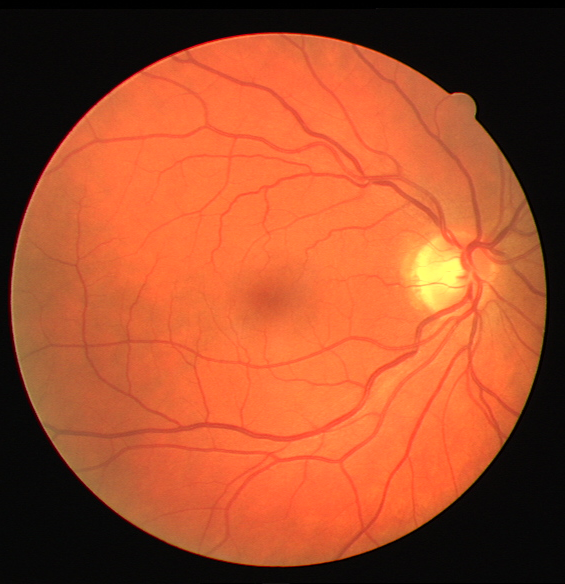
\includegraphics[width=0.3\columnwidth]{\figpath/retina/02_test} &
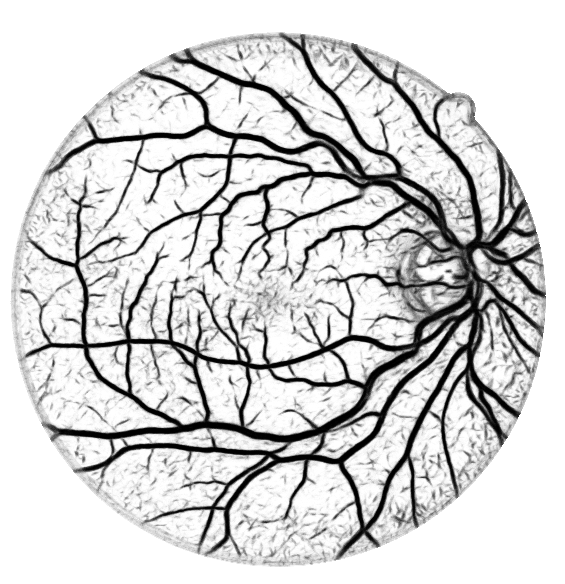
\includegraphics[width=0.3\columnwidth]{\figpath/retina/02_segmentation_gabor_inv.png} &
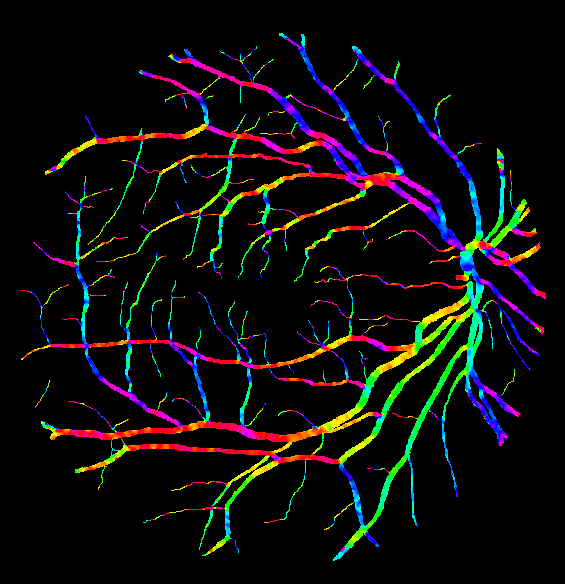
\includegraphics[width=0.3\columnwidth]{\figpath/retina/002_orientation_masked} \\
%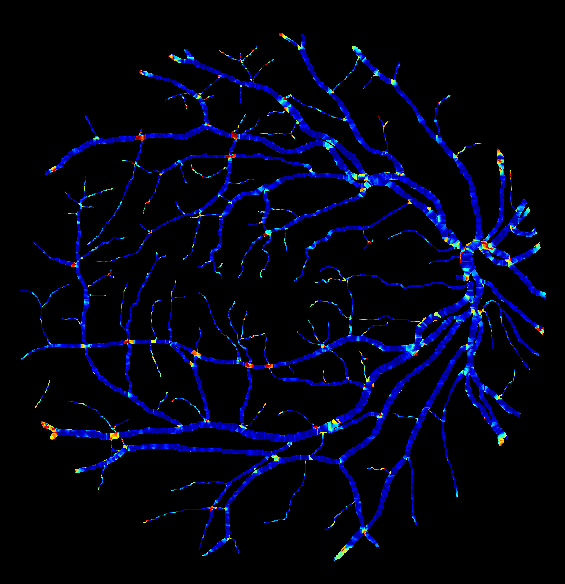
\includegraphics[height=0.15\textheight]{\figpath/retina/002_abs_error} \\
(a) & (b) & (c) \\
\noalign{\smallskip}
\end{tabular}
%
\caption{Estimating orientation in retinography: %
(a) input image; %
(b) segmentation of vessels by random forest classification of Gabor features; %
(c) orientation (indicated by colour) estimated using random regression over Gabor~features. The mask was not used to estimate orientation. %
%(c) magnitude of error (note the regions of high error at points of bifurcation.)
}
\label{f:retinography}
\end{figure}

% Specific aims of the study
Given an image, our aim is to determine where any linear structures exist in the image, and to measure values that correspond to low-level properties such as orientation, width, and cross-sectional profile. Although these properties form the basis of higher level, application-specific analysis (classifying structure as \emph{road}, \emph{rail} or \emph{river} in aerial photographs, for example), our focus is purely on computing the local attributes as accurately and robustly as possible; by improving the accuracy of the values we estimate, it follows logically that performance should improve for all higher level analysis methods that use these values as inputs.\footnote{Any algorithm that does not benefit from better input should be regarded with suspicion.}

%For example, any method to move from a map of vessel probabilities and predicted orientations in a retinograms, to an explicit grouping of pixels that belong to individual vessels, is likely to benefit from a priori knowledge of the spatial arrangement vessels in that image class and the physical model of how vessels grow and bifurcate. Such a method will therefore be very different from that needed to group a similar set of local information into the road, rivers etc present in an image for aerial analysis

With this focus, we have two objectives: extract, at every image location, structural information that is rich enough to capture the underlying image properties yet sparse enough to be computed efficiently; and combine this raw local information to predict output values of interest (such as orientation).


% Review other people's attempts at solving the problem, and why they are found wanting
\subsection{Related Work}
\comment{
There is no 3D analogue of the \dtcwt{}. Therefore, we should avoid 3D datasets and related work as much as possible - this paper is solely about the analysis of 2D image structures. This includes aerial photography, retinal images, fingerprints and palmprints, surface inspection, and possibly fibre analysis.
}

Because previous attempts at detecting and measuring curvilinear structures have been surveyed elsewhere, from the general~\cite{Papari_Petkov_IVC11} to the application-specific~\cite{Kirbas_Quek_ACMCS04,Lesage_etal_MIA09}, here we briefly review only a few papers in applications areas of specific interest. We will also discount the very basic detection methods that simply threshold an image~\cite{Jiang_Mojon_TPAMI03} and very complex methods that use techniques such as phase fields~\cite{Peng_etal_IJCV09}, leaving us free to focus on the most popular approaches that apply a bank of filters to the image before interpreting the responses in a way that accentuates the `lineness' at every pixel.

Early examples modelled a curvilinear structure as an image `ridge', typically defined using second order derivatives and formulated either as a Hessian problem~\cite{Frangi_etal_MICCAI98,Sato_etal_MIA98} or as responses to a derivative filter~\cite{Staal_etal_TMI04,Aylward_Bullitt_TMI02,Steger_TPAMI98,Koenderink_vanDoorn_TPAMI92}. Interpreting the responses to these filters used hand-crafted equations based on the differential geometry of the image `surface'~\cite{Frangi_etal_MICCAI98,Sato_etal_MIA98}.

With the maturing of machine learning, it was recognized that hand-crafting could be replaced by flexible statistical models whose parameters were optimized to agree with input-output training example pairs; Gaussian mixture models~\cite{Soares_etal_TMI06}, %
artificial neural networks~\cite{Marin_etal_TMI11,Minh_Hinton_ECCV10}, %
support vector machines~\cite{Ricci_Perfetti_TMI07,Gonzalez_etal_CVPR09}, and %
$k$-nearest neighbour classifiers~\cite{Staal_etal_TMI04} were all popular choices. Not only are these methods well-established and understood within machine learning, but a learnt statistical model can also accommodate different sensing modalities (with different noise properties) and other `stuff' that is hard to hand-craft, making the resulting algorithms more easily transferrable.

In addition, learnt statistical models can be applied to \emph{any} vector of image features to predict the quantity of interest, and are not tied to a particular feature type with specific theoretical properties. Furthermore, flexible statistical models permit the option to include hand-crafted, application-specific features where beneficial~\cite{Staal_etal_TMI04}. As a result, subsequent studies were free to use alternative filter banks and features based on %
matched filters or templates~\cite{Chaudhuri_etal_TMI89,Pechaud_etal_CVPR09,Dixon_Taylor_IPC79,Hoover_etal_TMI00,Ricci_Perfetti_TMI07}; %
derivatives of a first~\cite{Cai_Chung_MICCAI06} or higher than second~\cite{Gonzalez_etal_CVPR09} order; %
Gabor filters~\cite{Soares_etal_TMI06,Dabbah_etal_MIA11}; %
moments~\cite{Marin_etal_TMI11}; %
principal component analysis~\cite{Minh_Hinton_ECCV10}; %
wavelet transforms; %
and the monogenic signal. %
Some of these filter banks have been evaluated previously in a brief comparison~\cite{Ayres_Rangayyan_JEI07}, though the authors admit that not all filters were compared exactly on a like-for-like basis; our work builds on this comparison.

As well as permitting flexibility in the choice of input feature vector, learnt statistical predictors can be used to predict more than just the presence of a line. In recent studies, for example, orientation~\cite{Zwiggelaar_etal_TMI04,Ayres_Rangayyan_JEI07}, width~\cite{Steger_TPAMI98,Zwiggelaar_etal_TMI04} and multi-class labels~\cite{Zwiggelaar_etal_TMI04} have all been predicted from image feature vectors.

Other facets of tube detection and measurement are interesting though not directly relevant to this work: %
detecting lines at multiple scales~\cite{Lindeberg_IJCV98,Sato_etal_MIA98}; %
dealing with junctions and bifurcations where multiple lines meet at a point~\cite{Chen_etal_TPAMI00};
regularizing estimated lines via snakes~\cite{Laptev_etal_MVA00} or dynamic programming~\cite{Gruen}; %
and line following or tracking~\cite{Aylward_Bullitt_TMI02,Perez_etal_ICCV01}.



% Describe what we do, and why it is better than preceding works
\subsection{Our Contributions}
% Briefly outline our attempt at solving the problem, and why it should be better than the solutions that have preceded it
This paper presents three contributions that advance the current body of knowledge in the analysis of curvilinear image structures.

First, we provide a detailed comparison of commonly used image filter banks in the context of their suitability for extracting the local image information pertaining to curvilinear structure. In doing so, we describe the desirable properties of a suitable filter bank, therefore enabling us to make a principled choice that balances the richness of the extracted information against efficiency (both computational and storage). This analysis leads us to apply a previously unexploited image filter -- the dual-tree complex wavelet transform (\dtcwt{}) -- to the task of curvilinear feature analysis. The \dtcwt{} benefits from specific properties, such as efficiency and phase information, that address the shortcomings of existing popular image filters (\sref{s:filtering}).

Second, we investigate and compare supervised learning approaches that, after training on a set of (input feature vector, target label) example pairs, turn a previously unseen feature vector of filter responses at a given location into an estimated output value. Specifically, we include the Random Forest statistical method -- not investigated in any similar study of which we are aware -- to predict outputs, and compare this to techniques that have been previously used. For line detection (\ie~image segmentation), we show that a carefully selected filter bank, coupled with a modern learning method that is capable of dealing with non-linear data, produces results that match or exceed the state-of-the-art without relying on application-specific assumptions to boost performance. For orientation, we show how to formulate the learning problem such that angle wraparound is dealt with correctly, and in doing so produce\comment{ significantly} better estimates than existing methods that compute orientation analytically. In addition, we show how predicting output responses via machine learning allows us to estimate the error associated with the predictions, which we propose may in itself be of use in further processing.

Third, we explore the similarities and differences between these different approaches, and present empirical evidence of which work best in practice for applications including retinography~(\sref{s:retinography}), mammography~(\sref{s:mammography}) and [another?].

In all cases, we back up theoretical claims for filter performance with thorough experimental validation on both synthetic and real data. 

%Finally, if for a given image class we know of additional properties that will be useful to predict and that can be reliably labelled on our training data (for example, a further classification of structure in aerial images to roads and rivers) these can easily be added to our protocol. 





\clearpage
\section{Input Image Features}
\subsection{Filtering}
\label{s:filtering}
In this section we consider the theoretical requirements of a suitable filter bank, keeping foremost in our mind the application in which the responses will be used. That is the set of responses for any given structure pixel should be distinguishable from that of any background pixel; the filters should be directionally selective to predict orientation; likewise to predict structure width the responses should be selective across scale.

\begin{figure}[t]
\centering
\begin{tabular}{@{}c c c c@{}} % @{} removes padding around the edge of the table
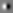
\includegraphics[width=0.2\columnwidth]{figs/filtering/Gx} &
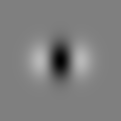
\includegraphics[width=0.2\columnwidth]{figs/filtering/Gxx} &
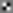
\includegraphics[width=0.2\columnwidth]{figs/filtering/Gxy} &
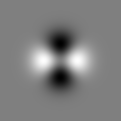
\includegraphics[width=0.2\columnwidth]{figs/filtering/Gxx-Gyy} \\
(a) & (b) & (c) & (d) \\
\noalign{\smallskip}
%
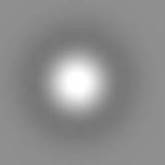
\includegraphics[width=0.2\columnwidth]{figs/filtering/mono_b} &
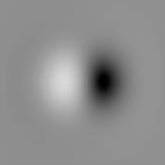
\includegraphics[width=0.2\columnwidth]{figs/filtering/mono_hx} &
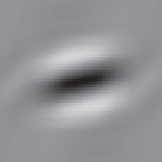
\includegraphics[width=0.2\columnwidth]{figs/filtering/dt_cwt_r4} &
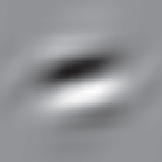
\includegraphics[width=0.2\columnwidth]{figs/filtering/dt_cwt_c4} \\
(e) & (f) & (g) & (h) \\
\noalign{\smallskip}
\end{tabular}
%
\caption{(a)~First derivatives $\Gx = \Gy^T$; (b-d)~Second derivatives, $\Gxx = \Gyy^T$, $\Gxy$; and $\Gxx-\Gyy$; (e,f)~Monogenic signal filters $B$ and $h_x = h_y^T$; (g,h)~Real and complex responses of the \dtcwt~ $15^\circ$ subband.}
\label{f:filters}
\end{figure}

\subsubsection{Gaussian derivatives}
\label{s:filtering_secondderivs}
%
We start by considering probably the most commonly used set of filters for linear structure detection (certainly within the context of vessel segmentation in medical images): derivatives of a Gaussian kernel.

Gaussian first derivatives - edge detection. Explain second derivatives.
%
The directional second-order derivative of a Gaussian generates an even (\ie~symmetric) image filter that resembles a bar or ridge feature. Like their first-order counterparts, second-order derivatives are steerable though they require three rather than two basis filters. The second-order basis filters are not separable, though a different formulation generates three equivalent basis filters -- $\Gxx$, $\Gyy$ and $\Gxy$ (\fref{f:filters_secondderivs}) -- that are. The response to a second-order derivative is given by
%
\begin{equation}
R(\theta) = \Ixx \cos^2(\theta) + \Iyy \sin^2(\theta) + \Ixy \sin(2\theta)
\label{e:secondderivs_response}
\end{equation}
%
\noindent where $\Ixx = \Gxx\ast I$, $\Iyy = \Gyy\ast I$ and $\Ixy = \Gxy\ast I$ are the responses to the three separable filters. This response function has four stationary points in the range $[0,2\pi)$, occuring at
%
\begin{equation}
\theta = \frac{1}{2} \tan^{-1}\left( \frac{2\Ixy}{\Ixx-\Iyy} \right).
\label{e:secondderivs_orientation}
\end{equation}
%
\noindent Two of these points, separated by $\pi\,\rad$ because the filter is rotationally symmetric, correspond to the directions in which the filter is aligned with the feature and the \emph{absolute} value of the response is maximal; the other two points correspond to the two perpendicular directions.

Because, however, the maximal absolute response may correspond to either a maximum or minimum (depending on whether the underlying feature is light-on-dark or vice versa) the only way to find out which of the two perpendicular directions has maximal absolute value is to evaluate the response at both and choose the direction corresponding to the larger absolute value. As a result, estimating orientation from second-order derivatives becomes a nonlinear problem.

Efficient approximations to computing second-order derivatives of the Gaussian can be achieved through Haar-like approximations to the derivative filters~\cite{Bay_etal_CVIU08} or by approximating the Gaussian filter and applying local finite differences~\cite{Kovesi_DICTA10}.

Note this approach is often reformulated by creating a Hessian matrix with the xx and yy derivates on the lead diagonal and the xy derivatives on the opposing diagonal. Solving this matrix produces eigen vectors with direction theta and thetaN and responses R.

G2D's work on the assumption that when steered to match the orientation of a structure, the response will be large, whilst the response in the perpendicular direction will be near-zero. Thus structures can be distinguished from flat backgrounds (both responses near-zero) or circular blob-like structures (both responses large). Equation () (or its Hessian reformulation) provides an elegant solution for determining this orientation analytically, from which the responses can be used to detect structure directly []. Alternatively the filters may be steered to multiple orientations over multiple scales and used as features in a machine learning algorithm [].

However, there are two problems in using second derivatives alone. Firstly, a strong edge in the image will produce an "echo" response that cannot be distinguished from the response at the centre of a CLS. This may seem an arbitrary construct; however it is easy find examples in real data. For example, the edge of the optic disc in a retinogram (Fig X) is often misclassified as a vessel, whilst similar artefacts may occur at the edges of lesions or near the pectoral muscle in mammograms.

Secondly, due to noise in the image, the symmetric profile of a CLS may be disrupted to the extent that not only does the equation [] produce inaccurate results, the responses themselves hold no usual information that a machine learning algorithm to take advantage of. Again, this can be seen clearly in real data, particularly in structures that have a width of only one or two pixels, such as the smallest vessels in retinograms.

The first problem tells us that it is not enough to only have filters designed to match the shape profile of the CLS we want to detect if such filters cannot distinguish other structures in the image background. The second problem shows we cannot rely on the assumptions we make about the CLS in real images. Combining both ideas motivates us to choose a filter bank that more generally represents an image. Our goal then is not to make a priori assumptions about how we want filters to respond to particular structures, but simply to ensure the set of filter responses produce a unique signature for differing structures. It is then up to our chosen machine learning algorithm to match the various signatures present in the training data to the output measure of interest.

Returning to Gaussian derivatives, we note the cause of both problems is that at a given scale and orientation, we can only compute the response to a filter with even symmetry. An intuitive solution is to supplement these filters with Gaussian 1st derivatives (as used most commonly in edge detection e.g. Canny) as used to heuristically discard edge echo responses in []. However, we prefer the solution recommended in [], using the Hilbert transform of the second derivatives. A steerable response can be computed from four separable basis filters, defined below:

The advantage of using Rh rover first derivatives is that it allows us to represent the responses as magnitude and phase:

We show in section X how this improves results, particularly for orientation (and width?) prediction.

\subsubsection{Gabor derivatives}
\label{s:filtering_gabor}
Next we consider Gabor filters.

A Gabor filter pair consists of one sine and one cosine function, in 2 dimensions and windowed with a Gaussian function. They are therefore directionally sensitive, and can also recover phase information from the underlying image region.

Because Gabor filters recover both orientation and phase information, they are a popular choice of filter in image processing applications~\cite{Daugman_TASSP88}. In general, however, they are neither separable nor steerable, although methods to approximate steerability have been explored~\cite{Teo_1987,Perona_PAMI95}. Therefore, they must be applied exhaustively over a discrete set of orientations which makes them expensive in terms of computation and (if all responses are to be stored simultaneously) memory.

%
\begin{equation}
g_{re}(x,y;\lambda,\theta,\sigma,\gamma) = \exp(-\frac{x'^2 + \gamma^2 y'^2}{2\sigma^2}\cos(2\pi \frac{x'}{\lambda})
\label{e:gabor_real}
\end{equation}
\begin{equation}
g_{im}(x,y;\lambda,\theta,\sigma,\gamma) = \exp(-\frac{x'^2 + \gamma^2 y'^2}{2\sigma^2}\sin(2\pi \frac{x'}{\lambda})
\label{e:gabor_imag}
\end{equation}
\begin{align}
x' = x\cos\theta + y\sin\theta \\
%
y' = -x\sin\theta + y\cos\theta
\label{e:gabor_xy}
\end{align}
%

As with Gaussian derivatives, these have been used extensively in detecting CLS, although again often only the even filter [eq X] is used as this is what is assumed will match the shape. For the same reason we match G2 with its Hilbert pair, we recommend using both odd and even parts, with maximum benefits obtained by combining them as a magnitude/phase pair and show experimentally the advantages of doing so in section X.

Note that unlike Gaussian derivatives, Gabor filters are neither separable nor steerable, making them much more expensive to compute. In contrast we now consider two further filtering schemes designed to measure magnitude and phase across and orientation and scale more efficiently: the monogenic signal; Gabor wavelets~\cite{Daugman_TASSP88}; and the Dual Tree Complex Wavelet Transform (\dtcwt{}~\cite{Kingsbury_PTRSLA99}), so far unexploited in applications analysing curvilinear structure.


\subsubsection{The Monogenic Signal}
\label{s:filtering_monogenic}
The monogenic signal~\cite{Felsberg_Sommer_TSP01} computes phase and orientation at a given image location using three filters: one even band-pass filter $B$, and an odd quadrature pair of filters $h_x(x,y) = x/f(x,y)$ and $h_y(x,y) = y/f(x,y)$ where $f(x,y) = 2\pi(x^2 + y^2)^{\frac{3}{2}}$ (\fref{f:filters_monogenic}). These filters are combined to compute local amplitude~($A$), phase~($\psi$) and orientation~($\theta$) at every location in the image:

\begin{align}
A       &= \sqrt{{I_B}^2 + {I_{hx}}^2 + {I_{hy}}^2}
\label{e:monogenic_amplitude} \\
%
\psi	  &= \tan^{-1}\left[ \frac{I_B}{\sqrt{{I_{hx}}^2 + {I_{hy}}^2}} \right]
\label{e:monogenic_phase} \\
%
\theta  &= \tan^{-1}\left[ \frac{I_{hy}}{I_{hx}} \right]
\label{e:monogenic_orientation}
\end{align}

\noindent where $I_B = I \ast B$, $I_{hx} = h_x \ast I_B$ and $I_{hy} = h_y \ast I_B$.

The local amplitude provides a magnitude of response that is consistent for all structures and orientations while the local phase provides a measure of symmetry (in a profile of the structure perpendicular to its orientation), varying from $-\pi/2$ for a negative line (\ie~a dark line on a light background), through $0$ for an edge, to $\pi/2$ for a positive line.

Though the monogenic signal combines both odd and even filters, the even filter $B$ is isotropic and therefore has no directional sensitivity. All orientation information therefore comes from the odd filters $h_x$ and $h_y$, such that orientation is not recovered for symmetric image features (\eg~at the centre of a bar or ridge).

\subsubsection{The Dual-tree Complex Wavelet Transform}
\label{s:filtering_dtcwt}

The Dual-Tree Complex Wavelet Transform (\dtcwt{}~\cite{Kingsbury_ACHA01}) is a directionally selective representation that combines the strengths of approximately shift-invariant coefficient magnitudes and local phase information with the computational efficiency of decimation (\ie~downsampling the image rather than increasing the filter size).

For a given pixel at a given scale, the \dtcwt{} combines the responses to a pairs of wavelets -- one real, one complex, and differing in phase by $90\deg$~(\fref{f:filters_dtcwt}) -- at six orientations: $\pm 15\deg$, $\pm 45\deg$ and $\pm 75\deg$. Because these filters are not exactly rotationally symmetric, the wave frequencies of the $\pm 45\deg$ sub-bands must be reduced so that they lie closer to those at $\pm 15\deg$ and $\pm 75\deg$, and all six sub-bands are adjusted so that the phase at the centre of the impulse response of each wavelet is zero~\cite{Kingsbury_ECSP06}.

% Multiresolution filtering
To compute filter responses at different scales, the image is repeatedly downsampled by a factor of two in every axis before applying the same six filter pairs again. To get the response for every scale at a given location on the original pixel grid, filter responses on a coarse grid at lower levels of the tree are interpolated with a bandpass method~\cite{Anderson_etal_ICIP05}.

% Advantages
The \dtcwt{} has the benefit of a low redundancy of just 4:1, making it feasible to store the decomposition of even large images. It is also efficient, relative to other methods such as Gabor filtering, through its use of downsampling.

% Disadvantages
Decimation does, however, introduce complications because the filters are not necessarily computed centrally over structures of interest. The phase of \dtcwt{} coefficients within the support of a structure therefore encodes both the symmetry of the structure and a spatial offset. By computing phase differences both spatially and across scale, however, it is possible both to recover local phase that is globally consistent for structure symmetry (and analogous to the phase returned from the monogenic signal) and to compute local orientation analytically~\cite{Anderson_ICIAR05,Anderson_SSP05}.

It is not clear, however, how to use responses to the \dtcwt{} filters to compute a single measure of curvilinear structure probability. Though we could select the maximum of the six oriented sub-band coefficients at each scale and combine them in a measure of phase congruency (as in a method based on the monogenic signal~\cite{Wai_etal_MICCAI04}), this would discard potentially useful information.

We therefore construct a feature vector that characterises each pixel by sampling \dtcwt{} coefficients from the six oriented sub-bands in each of the $s$ finest decomposition scales from a neighbourhood centred on the pixel, and transforming every complex response, $c$, to polar coordinates (\ie~magnitude, $|c|$, and angle, $\angle c$). Since orientation is only defined up to a rotation of $180^\circ$, however, the sign of the angle is arbitrary and so we use its absolute value, $|\angle c|$.

\subsubsection{Other stuff}
\label{s:filtering_extras}
Finally we acknowledge that there are of course many further filter banks we do not test in this paper, and for which an exhaustive comparison of results is unfeasible. However, we show that it is the properties we choose to implement for a given a filter bank (e.g. a magnitude/phase versus just an even/odd response, decimation versus increasing filter size, oversampling scales etc.) rather than the inherent properties of the filters that have the biggest effect in performance. In turn, given a set computational cost, this allows us to make an informed choice of suitable filter bank for any given data.

We also show that a filter bank selected given these general criteria can produce features that outperform features handcrafted for a particular application.

One interesting concept we do not test is the idea of learning an optimal set of arbitrary filters for a given set of images, as in []. However, we believe that such an approach is only beneficial if the filters are optimised with respect to the task they need to perform (in our case and in [], separating the responses for CLS and background pixels within a classifier) and cannot see how optimising with respect to some other task (such as reconstructing the image in a maximally sparse way) is intrinsically a desirable thing to do. That said a comparison with the results in [] would be desirable if quantitative results on the DRIVE and STARE datasets were made available.

\subsection{Composing feature vectors from filter responses}
\label{s:composing_features}
In this section we consider how, for any pixel, to combine the responses of a given filter bank into a feature vector. In the simplest form, we just concatenate the responses from the raw filters at all scales and orientations, however we also consider the following:

\subsubsection{Steering}
\label{s:composing_features_steering}
For the Gaussian derivatives (and their Hilbert transform), we can choose to steer the raw responses at each scale to a fixed set of directions spread evenly across the circle (e.g. in the same directions we apply the Gabor filterbank). This potentially produces features that can be more easily matched to the appropriate output measure and for experimentation purposes provides a more direct comparison to the Gabor and \dtcwt{} filter banks.

\subsubsection{Complex form}
\label{s:composing_features_complex}
As discussed in the previous section, for the Gaussian, Gabor and \dtcwt{} filter banks at a given scale and orientation we have a pair of responses that can be thought of as a complex number, where by custom we use the response to the even filter for the real part and the odd response for its imaginary counterpart. We can then choose either to include the real and imaginary parts as separate dimensions in the feature vectors or represent the pair of responses as magnitude and phase. The latter is arguably a more intuitive way to think of the responses - considering the image profile sampled at a given orientation and scale, the magnitude signifies if a feature is present in this 1D signal, whilst the phase tells us about the shape of the feature as it varies from a valley, to a step, to a ridge. Note also that if an image is rotated through 180 degrees, a complex response C = a+ib becomes C*=a-ib. Thus if we want to make our features responses ambivalent to 180 degree rotations we can use the absolute value of the imaginary part when computing phase.

\subsubsection{Rotation invariance}
\label{s:composing_features_rotation}
Given a set of responses at orientations spread evenly over the circle, a common approach is to select the orientation with maximal response and circular shift the remaining responses in the feature vector such that the maximal orientation for each feature vector occupies the same dimension. The intention is to produce feature vectors with rotational invariance thus collapsing the size of the feature space (proportional to the number of discrete orientations in the filter bank) and making it easier for the classifier to do its job. Whilst theoretically appealing we show in section X that this has no discernible benefit in practice. Note also, with responses over multiple scales, we can choose either to allow the responses in each scale to shift independently or choose a single maximum orientation (e.g. from the scale that produces maximum response) to circularly shift all scales. Here we take the former approach although we have experimented with both and found little difference in performance.

\subsubsection{Pooling neighbourhood responses}
\label{s:composing_features_neighbours}
In contrast to faffing with rotational invariance, a simple yet effective measure is to pool the responses from neighbouring pixels. Again we have experimented with more exotic sampling schemes in which we interpolate responses in a circular pattern about the pixel of interest, but have found that in practice simply sampling a 3x3 window of responses provides most benefit. Of course this increases the dimension of the feature vectors nine-fold, but with machine learning algorithms (such as random forests) designed to cope with large dimensional features and plenty of training data (which is nearly always the case in this set up given each pixel in an image is a sample and thus even a small set of images typically contain millions of samples) this needn't be a problem.

Flow chart�


\clearpage
\section{Target Output Labels}
Our approach to analyzing and understanding images containing linear structure is to use statistical learning methods to recognize patterns present in training data in order to predict useful information in previously unseen images. More specifically, we focus on three tasks: detecting linear structures in the image; discriminating between linear structures of different types (\eg~classifying ducts from spicules in mammograms); and measuring the orientation of linear structures. Though the input image features are common across all three tasks, the output label we wish to predict is task-dependent.

\subsection{Detecting Linear Structure}
\label{s:review_orientation}
%
At a low and intermediate level, knowing the orientation of curvilinear linear structure is important for steering computation~\cite{Sonka_99}, extracting profiles~\cite{Zwiggelaar_etal_TMI04,Staal_etal_TMI04}, grouping and tracking curvilinear features~\cite{Aylward_Bullitt_TMI02}, and directional filtering such as nonmaximal suppression and anisotropic diffusion~\cite{Perona_PAMI90}. 
%Estimating the local \emph{orientation} of curvilinear structure is also important, though the literature in this area is more limited~\cite{Freeman_Adelson_TPAMI91,Koenderink_vanDoorn_TPAMI92}.
Applications at a high level, however, are more diverse.

As well as knowing where the linear structures are, we may also wish to know where they are heading.
% Define the output labels in a detection (i.e. single class classification) task
%
When using a statistical classifier to discriminate between two classes only, the simplest approach assigns a target label of zero or one to examples of each class, respectively (\emph{background} and \emph{foreground}, for example).%

\subsection{Classifying Linear Structure}
\label{s:review_orientation}
%
At a low and intermediate level, knowing the orientation of curvilinear linear structure is important for steering computation~\cite{Sonka_99}, extracting profiles~\cite{Zwiggelaar_etal_TMI04,Staal_etal_TMI04}, grouping and tracking curvilinear features~\cite{Aylward_Bullitt_TMI02}, and directional filtering such as nonmaximal suppression and anisotropic diffusion~\cite{Perona_PAMI90}. 
%Estimating the local \emph{orientation} of curvilinear structure is also important, though the literature in this area is more limited~\cite{Freeman_Adelson_TPAMI91,Koenderink_vanDoorn_TPAMI92}.
Applications at a high level, however, are more diverse.

As well as knowing where the linear structures are, we may also wish to know where they are heading.%
The literature on classifying curvilinear structures in mammograms is limited. We are aware of one study that demonstrated the feasibility of distinguishing between different types of structure using cross-sectional profiles obtained from manually annotated curvilinear structures, but did not obtain very satisfactory results when the method was fully automated~\cite{Zwiggelaar_etal_TMI04}. We recently reported preliminary classification (but not detection) results using our current approach~\cite{Chen_etal_IWDM10}.

In mammography, however, we concentrated on the task of distinguishing between spicules (that are an indicator of malignancy) and other curvilinear structures, such as ducts, that are of little consequence.
%
% Define the output labels in a classification (i.e. multi-class classification) task
%
When using a statistical classifier to discriminate between $k>2$ classes, the target label we assign to examples from the $i$th class is $k$-vector whose $i$th element is $1$, and all other elements are $0$.%

\subsection{Measuring Orientation}
\label{s:measuring_orientation}
\label{s:review_orientation}
%
At a low and intermediate level, knowing the orientation of curvilinear linear structure is important for steering computation~\cite{Sonka_99}, extracting profiles~\cite{Zwiggelaar_etal_TMI04,Staal_etal_TMI04}, grouping and tracking curvilinear features~\cite{Aylward_Bullitt_TMI02}, and directional filtering such as nonmaximal suppression and anisotropic diffusion~\cite{Perona_PAMI90}. 
%Estimating the local \emph{orientation} of curvilinear structure is also important, though the literature in this area is more limited~\cite{Freeman_Adelson_TPAMI91,Koenderink_vanDoorn_TPAMI92}.
Applications at a high level, however, are more diverse.

As well as knowing where the linear structures are, we may also wish to know where they are heading.%
To address this problem, we assume that orientation can be expressed as a (typically nonlinear) function of the responses to a given set of filters. Theoretically, we know this to be true for some filter banks (\eg~second derivatives of a Gaussian), though there are some complications.

First, when filters are applied at more than one scale we must ensure that we use the responses from the best scale for the true line width; analytic methods~\cite{Karssemeijer_teBrake_TMI96,Mei_etal_IVC09} assume this is the scale with the greatest response, though this is not guaranteed in the presence of noise. Second, any analytic method that assumes noise to be additive and Gaussian may suffer when this is not the case; this is a particularly a risk in medical applications (\eg~ultrasound has multiplicative Rayleigh noise). Third, for some filter banks (such as the \dtcwt{}) an analytic solution is not available at all or is fiendishly complex at best.

\label{s:orientation_representation}
%
When orientation is considered as a continuous variable, it is appropriate to estimate its value by regression. (Classifiers may be used in instances where orientatation is discretized into a finite number of bins.) Orientation, however, violates a common assumption in that it does not live in a Euclidean space; adding $2\pi$ radians gives the same orientation, for example. Also, orientation (unlike \emph{direction}) is only defined over half the circle; orientations exactly $\pi$radians apart are also considered to be identical.

A different representation is therefore needed, and one that respects these two conditions uses a unit vector in the complex plane where the underlying angle is doubled such that two orientations exactly $\pi$radians apart are mapped to the same complex value~\cite{Mardia_Jupp_00}:

\begin{equation}
	t_k = \cos 2\theta_k + i\sin 2\theta_k
\end{equation}

% Difference between two orientations
Representing orientation as a complex vector also allows us to define a distance measure between two values -- an estimated value, $t_{est}$, and ground truth, $t_{gt}$, for example:

\begin{equation}
	2\theta_{err} = |\angle(t_{gt} \cdot t_{est}^*)|,
\end{equation}
%
\noindent where $t^*$ denotes the complex conjugate of $t$. This error metric therefore accounts for the circular nature of orientation in a principled way.

% Interpreting the mean vector and its magnitude
Taking the mean over a set of orientations gives a complex vector whose angle is twice the average orientation over the set, and whose magnitude,
%
\begin{equation}
D = \left| \frac{\sum{t_k}}{N} \right|,
\label{e:2d}
\end{equation}
%
\noindent defines the spread -- known as the \emph{angular dispersion} -- of the samples in the set~\cite{Mardia_Jupp_00}. By definition, $D$ reaches a maximum of $1$ when all $t_k$ are equal, and a minimum of $0$ when orientations are distributed uniformly about the circle or when the sample consists of pairs exactly $\pi \text{radians}$ apart. 


\clearpage
\section{Statistical Learning Methods}
Given a set of filter-bank outputs from different scales, the second step in estimating orientation is to combine them in some way. There are two basic approaches: to find the scale at which the total magnitude of response is greatest, and combine the different filter responses at that scale analytically~\cite{Karssemeijer_teBrake_TMI96,Mei_etal_IVC09}; or to use a regression learning approach to combine the filter responses across all scales and orientations~\cite{Berks_etal_IPMI11}.

In this work, we consider three classifiers of varying complexity: a linear classifier; a boosted classifier; and a Random Forest.

\subsection{Linear Classification}
\label{s:learning_linear}
\label{s:regression_linear}
Under a linear regressor, the predicted output is a weighed sum of the filter responses. Because the outputs are complex the regression coefficients are complex also, though this problem is equivalent to regressing over $\cos 2\theta$ and $\sin 2\theta$ independently.

\comment{We may want to reintroduce a note here that there are two solutions to the orientation, and that this cannot be estimated from a linear regression alone (at least for the double angle representations)}

%Under ideal conditions, applying this method to the real filters (\eg~first and second derivatives) should produce regression coefficients identical to those computed analytically.\comment{Not sure if that is entirely relevant}

%Since the linear regressor minimizes the mean squared error (in $\cos 2\theta$ and $\sin 2\theta$), the uncertainty in the prediction can be represented as an axis aligned Gaussian distribution in the complex plane. If the errors are equally distributed for both $\cos 2\theta$ and $\sin 2\theta$ -- and our experience suggests that they are typically close -- then the angular error (\ie~the angle subtended by isocontours of the Gaussian) is constant for an input of given magnitude; uncertainty is proportionally lower for inputs with larger magnitude, and vice versa. Since phase is limited to the range $[-\pi,\pi)$, however, the magnitude of the feature vector is strongly correlated with the magnitude (rather than phase) of the response to the \dtcwt{}. As a result, image features with high contrast that respond strongly to the \dtcwt{} have lower relative uncertainty (an intuitive result).\comment{This could be considered as 'discussion' and may not be relevant right here}


%\subsection{Logistic Classification}
%\label{s:learning_logistic}
%%Since we are predicting sin2T and cos2T, it makes sense to apply some limits to the values these can take. One possibility is to us logistic regression (usually used for classification) which can model a linear region for appropriately scaled targets or a sigmoidal output if necessary. We scale sin and cos to the range [0,1] to learn the regressor and apply the reverse transform on the predictions. This does not restrict outputs to be on (or within) the unit circle but within the unit square.
%
%This is slower to train since it requires iteratively reweighted least squares to minimize the objective function though adds little to testing times.
%Uncertainty will be tricky here

\subsection{Boosted Learning}
\label{s:learning_boosted}
Though straightforward, linear regression breaks down if the relationship between inputs and outputs is in fact nonlinear. Furthermore, the output of a linear regressor is unbounded even though in reality $-1 \leq \sin\theta,\cos\theta \leq 1$. We therefore investigate additive (or \emph{boosted}) regression models that can not only limit output but also capture any nonlinearities in the relationship between feature vector and orientation.

In this work we use an additive model composed of $N=100$ piecewise constant functions. To train the model, we start with a zero residual and iterate the following steps $N$ times: fit a weak predictor to each dimension of the training data in turn; select the dimension and corresponding predictor that minimize the residual error; add a fraction (we use $0.05$) of the prediction to the estimated outputs -- a process known as \emph{shrinkage}~\cite{Friedman_AoS01}; and recompute the residual error. This boosting process is thought to be more insensitive to overtraining than most Machine Learning methods.

%

\subsection{Random Forests}
\label{s:learning_forest}
% Start by explaining how a single tree predicts a label (either discrete or continuous) from an input
Decision Trees -- a well-established and popular approach to Machine Learning -- are easy to understand and implement, and are capable of learning complex, nonlinear relationships over large numbers of variables (with absolute scales that are incommensurate) at a modest computational cost. 

A typical training algorithm for a classification and regression tree (CART~\cite{}) iteratively partitions the input space in order to optimize some splitting metric until a termination criterion is satisfied. The input feature vectors may then be discarded and the tree used as a lookup table where the output labels assigned to each leaf can be retained (and later sampled) or replaced by a description of their distribution (\eg~mean and variance) to reduce memory use. Both representations permit multimodal distributions (which is useful at points where lines cross or bifurcate) and a measure of confidence in the prediction of a previously unseen example.

\comment{Measure of confidence?}

%Splitting criterion
When determining how to partition the input space, all distinct partitions (based on threshold applied to an input feature) of the examples at a given node are ranked based on a measure of `goodness of split'. As an example, consider the average variance over the two potential partitions in question: the variance is minimized at the point where the data set is split with the minimum ovelap.

%Termination criterion
The examples assigned to every leaf are split repeatedly until some termination criterion is satisfied. One approach is to continue splitting the data until every leaf contains samples with exactly the same label (a `pure' leaf node). Leaves can later be merged -- a process known as `pruning' -- for efficient lookup at run-time. We have found (as have others~\cite{Criminisi_MICCAI11}), however, that it is computationally more efficient and more robust to stop based on measure of spread within the two proposed leaves (we use 0.05\% of the total variance over all output labels). One further advantage of avoiding pure leaf nodes is that each leaf contains several training samples such that we can estimate the distribution over output labels for every leaf, thus providing a measure of confidence in the prediction that varies over the input space.


[One advantage of the (pruned) tree approach is that each bin contains a number of training samples such that we can estimate a mean value and an uncertainty (variance) for every leaf. In other words, the variance is very much data dependent.]
% Details on how a Random Forest works for either classification or regression
\label{s:rf_background}

% Then explain how sampling from the training examples and the input features, reduces correlation between trees such that a 'forest' of them produces better results

Using an ensemble of $F$ different trees (dubbed a \emph{Random Forest}~\cite{Breiman_ML01}), improves performance by reducing correlation between the outputs of the trees. Specifically, the forest produces $F$ predictions whose distribution can be used directly or averaged (using the individual measures of spread as weights if available).

The key to the Random Forest's performance is that every tree is built using randomly selected input features from randomly selected examples. For every partition at every level of the tree, only a random subset of $m < M$ input dimensions are considered rather than assessing all $M$ inputs. Similarly, $F$ bootstrap sets of $N$ examples are generated by sampling with replacement from the (finite) training data; if a generative model is available, a different training set can be synthesized for each tree without sampling.

As well as giving state of the art performance in a number of applications~\cite{Criminisi}, Random Forests also have relatively few parameters to tune and are often resistant to overtraining.

% Details on how a Random Forest works specifically for detection
%
During classification, an unseen feature vector is classified independently by each tree in the forest; each tree casts a unit class vote, and the most popular class can be assigned to the input vector. Alternatively, the proportion of votes assigned to each class can be used to provide a probabilistic labelling of the input vector.
% Points specific to estimating orientation with a Random Forest
When using a Random Forest as a regressor to predict orientation, we must take special care to ensure that the sample statistic (\eg~variance) used to partition the training data is appropriate. One statistic that does respect the circular nature of orientation is the angular dispersion, and so it is a natural choice for choosing an optimal partition of the sample.

When using a pruned tree, we can replace the samples at each leaf by a histogram that captures  any multimodal properties of the output (where lines cross, for example). Alternatively, we can replace the samples at each leaf by their summary statistics to save memory. In the case of orientation, the mean of the complex values gives both the average orientation (the angle of the mean vector) and the angular dispersion of the sample (the magnitude of the mean vector). This therefore provides a measure of confidence in the estimate for a single tree (in contrast to when using unpruned trees where every estimate has an identical confidence of 1).

When computing the final output of the forest, we can also take the mean over all $F$ outputs to give an estimate of orientation that is weighted by the confidence in each individual prediction. This output vector will also have a magnitude in the range $[0,1]$ that indicates confidence in the overall prediction produced by the forest.
%

Considering that curvilinear structure has a well-defined orientation, the confidence in an orientation estimate can also be used as a substitute for detection.

\subsection{Sampling Data}
\label{s:learning_sampling_data}
The final step in our method is to determine how we sample data for the forests. We have two schemes, one for running experiments on training data (e.g. to evaluate parameter options), the other for making final predictions on test data.
In the first scheme, we simply take some fixed size random subsample of pixels across the whole training data, with an equal number of background and foreground pixels (although only the foreground pixels are used orientation and width prediction). We then take a bootstrap sample of this data to train each tree in the forest. To test the forest, we take a second subsample from the pixels in the main training data not used in the first set. We can repeat this scheme, taking different random subsamples at every iteration, to compute a measure of uncertainty in prediction performance.
To make final predictions on the test data, we adopt a slightly more complicated sampling scheme that aims to better use all the data in the training set. In the first stage, we sample a different random subset of the training data for each tree during forest building, recording which pixels were selected. We then use the forest to predict all the training data, where at each pixel we aggregate only those predictions from trees for which the pixel wasn't selected. We can thus produce an unbiased prediction error at each pixel, analogous to the out-of-bag error described in Breiman's original random forest work [].
We then build a second forest, where again we sample a different random subset of the training data for each tree, only this time rather than uniformly sampling from the data, we weight the samples according to equation X,
%
\begin{equation}
Er = x
\label{e:reweight_sampling}
\end{equation}
%
where Ep is the prediction error described above and is defined separately for detection, orientation and width prediction as follows:
%
\begin{align}
E   &= a
\label{e:reweight_detect} \\
%
E	&= b
\label{e:reweight_orientation} \\
%
E   &= c
\label{e:reweight_width}
\end{align}
%
This has the effect of oversampling pixels that were poorly predicted in the first forest (with lambda controlling the level of oversampling versus uniform sampling) and results in a significant improvement in overall prediction performance. Note that the second stage of this process can be repeated to determine a suitable value for lambda. Indeed subject to time constraints, we could iterate until our predictions in the training data converge. In practice however, we evaluate performance for a fixed set of values for lambda and select the best.
The resulting forest can then be used to make predictions for all images in the test data.


\clearpage
\section{Data \& Applications}
We evaluate our methods on three real datasets, two of which containing retinograms and the third containing images of the?. These data are described below.
%
\subsection{DRIVE}
\label{s:dataset_drive}
%
% Briefly describe the disease, and give figures for its prevalence or incidence, and estimated economic costs if available. 
An estimated XXX people suffer from diabetes in the US~\cite{source} and YYY in the UK~\cite{source}, and these numbers are rising. Of those suffering from diabetes, approximately Z\% will suffer from diabetic retinopathy -- the leading cause of legal blindness in people aged 20-74 in the United States, with an estimated annual cost of \$500 million in the US alone~\cite{Zhang_etal_JAMA10}.
\cite{Thomas_etal_BMJ12}.

% Also describe how (human) image analysis is used to improve treatment and reduce these costs.
Early diagnosis and treatment is key to improving quality of life and reducing the economic impact of the disease, and one way to diagnose retinopathy is by analysing images of the retina taken with a fundus camera. Indicators of retinopathy that are visible in the fundus image include presence of microaneurysms, haemorrhages and small patches of fat (exudates), variation in width along the vessels (venous beading), and the formation of new vessels (neovascularization). 

\label{s:review_orientation_retinography}
%
The rate of change of orientation (tortuosity) of blood vessels in a retinogram can serve as a diagnostic indicator of vascular disease such as retinopathy of prematurity~\cite{Wallace_TAOS07,Hart_etal_IJMI99}. Though studies suggest that vessels can be detected and segmented~\cite{Staal_etal_TMI04,Ricci_Perfetti_TMI07}, few have addressed the problem of measuring their orientation and quantifying tortuosity.


\label{s:review_orientation_retinography}
%
The rate of change of orientation (tortuosity) of blood vessels in a retinogram can serve as a diagnostic indicator of vascular disease such as retinopathy of prematurity~\cite{Wallace_TAOS07,Hart_etal_IJMI99}. Though studies suggest that vessels can be detected and segmented~\cite{Staal_etal_TMI04,Ricci_Perfetti_TMI07}, few have addressed the problem of measuring their orientation and quantifying tortuosity.

%

The publicly available DRIVE dataset~\cite{Staal_etal_TMI04} contains 40 full colour, JPEG compressed retinogram images (\fref{f:retinography}a) that originate from a diabetic neuropathy screening program in The Netherlands, where subjects were aged 25-90. The images were acquired using a Canon CR5 non-mydriatic 3CCD camera with a 45 degree field of view (FOV) and 8 bits per colour plane, and are $768 \by 584$ pixels in size. The field of view is defined by a mask, provided with every image, that results in a cropped image $565 \by 584$ pixels in size.

Forty images from a total of 400 were selected for the dataset, seven of which exhibit signs of mild early diabetic retinopathy. These 40 are split into 20 training and 20 test images. Every image comes with at least one mask (test images have two), hand-labelled by human observers, that define ground truth vessel segmentations (\fref{f:fig_drive_examples}).

\subsection{STARE}
\label{s:dataset_stare}
STARE is basically the same as DRIVE. What more can I say?

\subsection{Fibre}
\label{s:dataset_stare}

\subsection{Synthetic images}
\label{s:dataset_synthetic}

In addition, we use synthetic data to explicate particular points discussed in section X. Each synthetic image is created as follows:
Generate a line of random direction, contrast and width, with elliptical profile centred in 64x64 background. The background may either be flat or containing an edge of random orientation and contrast. The image is then corrupted by signal dependent Rician noise, subject to equation X.
%
\begin{equation}
I_{noise} = I
\label{e:rician_noise}
\end{equation}
%


\clearpage
\section{Experiments \& Results}
\label{s:experiments}

We first show use sets of synthetic data with increasing noise to highlight the benefit of learning to predict orientation as opposed to relying on analytical methods (we take it as given now that learning is established as superior to analytical methods for detecting structure), and to examine the benefit of using both odd and even filters.
We then test all combinations of composing feature vectors from our four filter banks using subsamples of the training data for each real dataset.
Finally, we use the best performing feature vector composition and construct forests to apply to the test data for the DRIVE (and STARE?) data as described in section X, and compare the results to previous work.

\subsection{Experiment 1: Synthetic data, increasing noise}
\label{s:experiments_1}
Figures:
\begin{itemize}
  \item Percentage of correctly selected oriented sub-band as noise increases
  \item Percentage of correctly selected scale as noise increases
  \item Overall Gaussian prediction error
  \item The same for DRIVE data
  \item Performance for individual scales
\end{itemize}
%	
Key point: analytic solutions don't effectively compile information of all scale - you are better off picking a single scale. In contrast, learning methods improve as all scales are included. Note also that including all scales provides a more consistent performance over structures of all widths*

\subsection{Experiment 2: Synthetic data, Line vs Edge }
\label{s:experiments_2}
[may leave out or combine with 1]
%
\begin{itemize}
  \item Line detection when on edge: with/without odd component, 1x1 vs 3x3
  \item Performance specifically at edge:

  %
  \begin{itemize}
    \item Show figure on synthetic data
    \item Real example from DRIVE data
  \end{itemize}
  %
\end{itemize}
%
\begin{figure}[t]
\centering
\begin{tabular}{@{}c c c@{}}
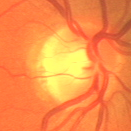
\includegraphics[width=0.3\columnwidth]{\figpath/retina/02_optic} &
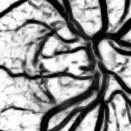
\includegraphics[width=0.3\columnwidth]{\figpath/retina/02_optic_g2d_inv} &
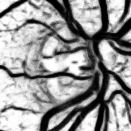
\includegraphics[width=0.3\columnwidth]{\figpath/retina/02_optic_g12d_inv} \\
%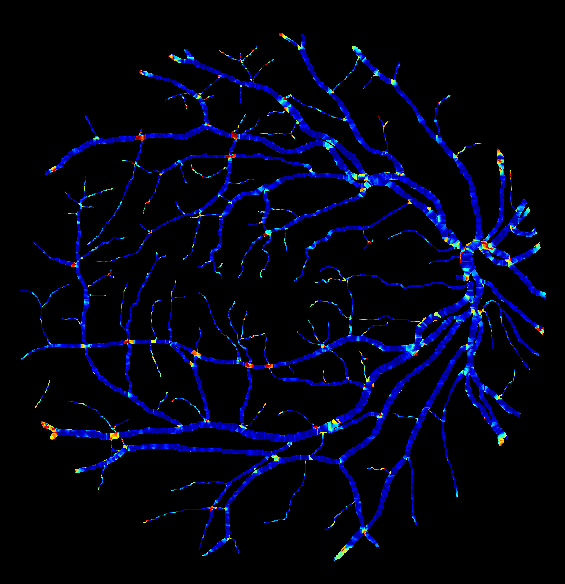
\includegraphics[height=0.15\textheight]{\figpath/retina/002_abs_error} \\
(a) & (b) & (c) \\
\noalign{\smallskip}
\end{tabular}
%
\caption{Detecting vessels in retinography: %
(a) Magnified region containing optic disk; %
(b) Segmentation using only even filter responses as features: the false positive predictions
at the edge of the disk have similar strength to neighbouring vessels; %
(c) Segmentation using odd and even filter responses: false positives are still present, but at a
much lower strength to nearby vessels;
}
\label{f:retinography}
\end{figure}

\subsection{Experiment 3: Comparing Filters banks and Feature Vector Compositions}
\label{s:experiments_3}
Experiment 3 - real data, all permutations of composing feature vectors
%
\begin{table*}[t]
\centering
\small
\begin{tabularx}{\linewidth}{X X r r r r}
\toprule
\multicolumn{6}{l}{Retinograms: DRIVE data} \\
\midrule
            &
            & \multicolumn{2}{c}{Vessel Detection \linebreak ($A_z$)}
            & \multicolumn{2}{c}{Vessel Orientation \linebreak ($mae$)}  \\
            &           & $w = 1$         & $w = 3$         &   $w = 1$       &   $w = 3$   \\
\midrule
\multirow{3}{3cm}{ Gaussian }
            & $G$         & 0.947 $\pm$ 6.4* & 0.959 $\pm$ 5.3   & 6.89 $\pm$ 0.042  & 6.04 $\pm$ 0.037 \\
            & $H$         & 0.838 $\pm$ 11.0& 0.957 $\pm$ 6.4   & 10.7 $\pm$ 0.046  & 6.62 $\pm$ 0.031 \\
            & $G, H$      & 0.958 $\pm$ 6.4 & 0.961 $\pm$ 6.0  & 6.67 $\pm$ 0.050  & 5.96 $\pm$ 0.028 \\
\midrule
\multirow{3}{3cm}{Gaussian, \newline steered to 6 directions}
            & $G$         & 0.949 $\pm$ 5.0 & 0.961 $\pm$ 5.5  & 6.71 $\pm$ 0.038  & 5.91 $\pm$ 0.022 \\
            & $H$         & 0.838 $\pm$ 10.8& 0.956 $\pm$ 5.7   & 10.39 $\pm$ 0.063  & 6.55 $\pm$ 0.029 \\
            & $G,H$       & 0.959 $\pm$ 5.7 & 0.962 $\pm$ 5.8  & 6.46 $\pm$ 0.031  & 5.85 $\pm$ 0.026 \\
\midrule
\multirow{3}{3cm}{Gabor, \newline 6 directions}
            & $Re$      & 0.948 $\pm$ 6.0   & 0.960 $\pm$ 5.7  & 6.15 $\pm$ 0.033 & 5.47 $\pm$ 0.021 \\
            & $Im$      & 0.854 $\pm$ 1.2   & 0.953 $\pm$ 6.5   & 8.08 $\pm$ 0.041 & 5.52 $\pm$ 0.024 \\
            & $Re,Im$   & 0.959 $\pm$ 5.5   & 0.962 $\pm$ 5.7  & 5.82 $\pm$ 0.027 & 5.34 $\pm$ 0.019 \\
\midrule
\multirow{3}{3cm}{\dtcwt{}}
            & $Re$      & 0.920 $\pm$ 7.7   & 0.951 $\pm$ 6.1  & 7.08 $\pm$ 0.026 & 5.78 $\pm$ 0.023 \\
            & $Im$      & 0.900 $\pm$ 6.9   & 0.951 $\pm$ 6.6  & 7.76 $\pm$ 0.046 & 5.70 $\pm$ 0.028 \\
            & $Re,Im$   & 0.952 $\pm$ 5.6   & 0.956 $\pm$ 5.9  & 5.92 $\pm$ 0.024 & 5.51 $\pm$ 0.027 \\

\bottomrule
\noalign{\smallskip}
\end{tabularx}

\caption{Detecting and predicting the orientation of retinal vessels. DRIVE database, training images:
effect of pooling neighbourhood filter responses.}
\label{t:drive_training_1}
\end{table*}
%
\begin{table*}[t]
\centering
\small
\begin{tabularx}{\linewidth}{p{3cm} X X X X r r}
\toprule
\multicolumn{7}{l}{DRIVE data} \\
\midrule
            &
            & $w$
            & Size
            & Time
            & \multicolumn{1}{c}{Vessel Detection \linebreak ($A_z$)}
            & \multicolumn{1}{c}{Vessel Orientation \linebreak ($mae$)}  \\

\midrule
\multirow{6}{3cm}{ \textbf{Gaussian}, 
    \newline separable filters, $G_\sigma$, $H_\sigma$, 
    \newline  $\sigma = [1 2 4 8 16]}
        & $G$                   & \multirow{3}{1cm}{ 1 }
                                    &      15   &  3     & 0.947 $\pm$ 6.4 & 6.89 $\pm$ 0.042   \\
        & $H$                       &&     20   &  4     & 0.838 $\pm$ 11.0& 10.67 $\pm$ 0.046  \\
        & $G, H$                    &&     35   &  7     & 0.958 $\pm$ 6.4 & 6.67 $\pm$ 0.050   \\
        & $G$                   & \multirow{3}{1cm}{ 3 }
                                    &     135   &  3      & 0.959 $\pm$ 5.3 & 6.04 $\pm$ 0.037 \\
        & $H$                       &&    180   &  4      & 0.957 $\pm$ 6.4 & 6.62 $\pm$ 0.031 \\
        & $G, H$                    &&    315   &  7      & 0.961 $\pm$ 6.0 & 5.96 $\pm$ 0.028 \\

\midrule
\multirow{13}{3cm}{\textbf{Gaussian}, \newline steered to 6 directions}
        & $G$                   & \multirow{3}{1cm}{ 1 }
                                    &      30   &  3     & 0.949 $\pm$ 5.0   & 6.71 $\pm$ 0.038 \\
        & $H$                       &&     30   &  4     & 0.838 $\pm$ 10.8   & 10.39 $\pm$ 0.063\\
        & $G,H$                     &&     60   &  7     & 0.959 $\pm$ 5.7   & 6.46 $\pm$ 0.031 \\
        & $G$                   & \multirow{3}{1cm}{ 3 }
                                    &     270   &  4      & 0.961 $\pm$ 5.5   & 5.91 $\pm$ 0.022 \\
        & $H$                       &&    270   &  5      & 0.956 $\pm$ 5.7   & 6.55 $\pm$ 0.029 \\
        & $G,H$                     &&    540   &  9      & 0.962 $\pm$ 5.8   & 5.85 $\pm$ 0.026 \\

        & $Mag$                     &&    270   & 11    & 0.932$\pm$7.6     & 5.82$\pm$0.023 \\
        & $Phase$                   &&   270    & 11    & 0.925$\pm$6.5    & 6.50$\pm$0.043 \\
        & $Mag, Phase$              &&   540    & 11    & 0.961$\pm$5.6     & 5.73$\pm$0.015 \\
        & \ldots using $|Im|$       &&   540    & 11    & 0.962$\pm$4.7     & 5.68$\pm$0.020 \\
        & \ldots rotated            &&   540    & 11       & 0.960$\pm$5.4     & --- \\
        & \ldots interpolated       &&   540    &  7      & 0.959$\pm$4.6     & 6.06$\pm$0.034 \\
        & \ldots additional scales  &&  1728    &  ?      & 0.962$\pm$4.7     & 5.58$\pm$0.025 \\
        & \ldots additional directions&&  1620  &  ?    & 0.962$\pm$4.6     & 5.62$\pm$0.027 \\

\midrule
\multirow{13}{3cm}{Gabor, \newline 6 directions}
        & $Re$                  & \multirow{3}{1cm}{ 1 }
                                    &      30   & 82   & 0.948 $\pm$ 6.0   & 6.15 $\pm$ 0.033 \\
        & $Im$                      &&     30   & 82   & 0.854 $\pm$ 1.2   & 8.08 $\pm$ 0.041  \\
        & $Re,Im$                   &&     60   &164 & 0.959 $\pm$ 5.5   & 5.82 $\pm$ 0.027 \\
        & $Re$                  & \multirow{3}{1cm}{ 3 }
                                    &     270   & 82   & 0.960 $\pm$ 5.7   & 5.47 $\pm$ 0.021 \\
        & $Im$                      &&    270   & 82   & 0.953 $\pm$ 6.5   & 5.52 $\pm$ 0.024 \\
        & $Re,Im$                   &&    540   &164 & 0.962 $\pm$ 5.7   & 5.34 $\pm$ 0.019 \\
        & $Mag$                     &&    270   &164  & 0.932$\pm$8.6     & 4.92$\pm$ 0.023 \\
        & $Phase$                   &&   270    &164  & 0.912$\pm$8.6     & 9.38$\pm$ 0.059 \\
        & $Mag,Phase$               &&   540    &164  & 0.959$\pm$5.9     & 4.93$\pm$ 0.015 \\
        & \ldots using $|Im|$       &&   540    &164  & 0.962$\pm$6.6     & 4.85$\pm$ 0.020 \\
        & \ldots rotated            &&   540    &164   & 0.963$\pm$4.7     & --- \\
        & \ldots interpolated       &&   540    & 10      & 0.959$\pm$5.0     & 5.44$\pm$0.022 \\
        & \ldots additional scales  &&  1728    &?      & 0.963$\pm$5.5     & 4.59$\pm$0.017 \\
        & \ldots additional directions&&  1620  &?    & 0.963$\pm$5.8     & 4.74$\pm$0.021 \\

\midrule
\multirow{11}{3cm}{\dtcwt{}}
        & $Re$                  & \multirow{3}{1cm}{ 1 }
                                    &      30   &{<}1  & 0.920 $\pm$ 7.7   &  7.08 $\pm$ 0.026  \\
        & $Im$                      &&     30   &{<}1  & 0.900 $\pm$ 6.9   &  7.76 $\pm$ 0.046 \\
        & $Re,Im$                   &&     60   &  1    & 0.952 $\pm$ 5.6   &  5.92 $\pm$ 0.024 \\
        & $Re$                  & \multirow{3}{1cm}{ 3 }
                                    &     270   &  6    & 0.951 $\pm$ 6.1   & 5.78 $\pm$ 0.023 \\
        & $Im$                      &&    270   &  6    & 0.951 $\pm$ 6.6   & 5.70 $\pm$ 0.028 \\
        & $Re,Im$                   &&    540   & 12  & 0.956 $\pm$ 5.9   & 5.51 $\pm$ 0.027 \\

        & $Mag$                     &&   270    & 12   & 0.918$\pm$7.2     & 5.05$\pm$ 0.02 \\
        & $Phase$                   &&   270    & 12   & 0.879$\pm$7.9     & 10.8$\pm$ 0.063 \\
        & $Mag,Phase$               &&   540    & 12   & 0.955$\pm$5.9     & 4.98$\pm$ 0.026 \\
        & \ldots using $|Im|$       &&   540    & 12   & 0.953$\pm$5.9     & 4.96$\pm$ 0.024 \\
        & \ldots rotated            &&   540    & 12    & 0.946$\pm$6.0     & --- \\
\midrule
\multicolumn{2}{l}{Monogenic}       & \multirow{1}{1cm}{ 3 }
                                    &    135    &  5      & 0.951$\pm$5.5     & 7.85$\pm$0.045 \\
\midrule
\multicolumn{2}{l}{All filters}     & \multirow{1}{1cm}{ 3 }
                                    &   1755    &?       & 0.964$\pm$5.0     & 4.63$\pm$0.024 \\

\bottomrule
\noalign{\smallskip}
\end{tabularx}

\caption{Detecting and predicting the orientation of retinal vessels. DRIVE database, training images:
effect of pooling neighbourhood filter responses.}
\label{t:drive_training_c}
\end{table*}
%
\begin{table*}[t]
\centering
\small
\begin{tabularx}{\linewidth}{p{3cm} X X X X r r}
\toprule
\multicolumn{7}{l}{Fibre data} \\
\midrule
            &
            & $w$
            & Size
            & Time
            & \multicolumn{1}{c}{Vessel Detection \linebreak ($A_z$)}
            & \multicolumn{1}{c}{Vessel Orientation \linebreak ($mae$)}  \\

\midrule
\multirow{6}{3cm}{ Gaussian }
            & $G$                   & \multirow{3}{1cm}{ 1 }
                                    &      15 &$(3, {<}1, 3)$     & 0.896 $\pm$ 3.2 & 8.82 $\pm$ 0.16   \\
            & $H$                   &&     20 &$(4, {<}1, 4)$     & 0.819 $\pm$ 1.8 & 16.60 $\pm$ 0.47  \\
            & $G, H$                &&     35 &$(7, {<}1, 7)$     & 0.901 $\pm$ 3.0 & 8.68 $\pm$ 0.17   \\
            & $G$                   & \multirow{3}{1cm}{ 3 }
                                    &     135 &$(3, {<}1, 3)$      & 0.902 $\pm$ 3.2 & 8.43 $\pm$ 0.17 \\
            & $H$                   &&    180 &$(4, {<}1, 4)$      & 0.892 $\pm$ 2.7 & 8.98 $\pm$ 0.24 \\
            & $G, H$                &&    315 &$(7, {<}1, 7)$      & 0.903 $\pm$ 3.0 & 8.32 $\pm$ 0.17 \\

\midrule
\multirow{6}{3cm}{Gaussian, \newline steered to 6 directions}
            & $G$                   & \multirow{3}{1cm}{ 1 }
                                    &      30 &$(3, {<}1, 3)$     & 0.897 $\pm$ 3.2   & 8.76 $\pm$ 0.16 \\
            & $H$                   &&     30 &$(4, {<}1, 3)$     & 0.820 $\pm$ 1.9   & 16.10 $\pm$ 0.43\\
            & $G,H$                 &&     60 &$(7, {<}1, 7)$     & 0.901 $\pm$ 3.0   & 8.60 $\pm$ 0.16 \\
            & $G$                   & \multirow{3}{1cm}{ 3 }
                                    &     270 &$(3, 1, 4)$      & 0.903 $\pm$ 3.1   & 8.40 $\pm$ 0.16 \\
            & $H$                   &&    270 &$(4, 1, 5)$      & 0.892 $\pm$ 2.8   & 8.85 $\pm$ 0.23 \\
            & $G,H$                 &&    540 &$(7, 2, 9)$      & 0.903 $\pm$ 2.9   & 8.31 $\pm$ 0.16 \\
\midrule
\multirow{3}{3cm}{Gabor, \newline 6 directions}
            & $Re$                  & \multirow{3}{1cm}{ 1 }
                                    &      30 &$(82, {<}1, 82)$   & 0.901 $\pm$ 3.1   & 7.92 $\pm$ 0.15 \\
            & $Im$                  &&     30 &$(82, {<}1, 82)$   & 0.835 $\pm$ 2.2   & 13.1 $\pm$ 0.4  \\
            & $Re,Im$               &&     60 &$(163, {<}1, 164)$ & 0.906 $\pm$ 3.0   & 7.75 $\pm$ 0.15 \\
            & $Re$                  & \multirow{3}{1cm}{ 3 }
                                    &     270 &$(82, {<}1, 82)$   & 0.907 $\pm$ 3.1   & 7.64 $\pm$ 0.13 \\
            & $Im$                  &&    270 &$(82, {<}1, 82)$   & 0.895 $\pm$ 3.0   & 7.87 $\pm$ 0.23 \\
            & $Re,Im$               &&    540 &$(163, {<}1, 164)$ & 0.908 $\pm$ 3.0   & 7.51 $\pm$ 0.13 \\
\midrule
\multirow{3}{3cm}{\dtcwt{}}
            & $Re$                  & \multirow{3}{1cm}{ 1 }
                                    &      30 & $({<}1, {<}1, {<}1)$  & 0.897 $\pm$ 3.0   &  8.07 $\pm$ 0.14  \\
            & $Im$                  &&     30 & $({<}1, {<}1, {<}1)$  & 0.834 $\pm$ 2.4   &  13.4 $\pm$ 0.42 \\
            & $Re,Im$               &&     60 & $({<}1, 1, 1)$    & 0.902 $\pm$ 3.0   &  7.91 $\pm$ 0.15 \\
            & $Re$                  & \multirow{3}{1cm}{ 3 }
                                    &     270 & $({<}1, 6, 6)$    & 0.903 $\pm$ 3.0   & 7.80 $\pm$ 0.14 \\
            & $Im$                  &&    270 & $({<}1, 6, 6)$    & 0.891 $\pm$ 3.0   & 8.06 $\pm$ 0.21 \\
            & $Re,Im$               &&    540 & $({<}1, 11, 12)$  & 0.905 $\pm$ 2.9   & 7.65 $\pm$ 0.13 \\

\midrule
\multirow{6}{2cm}{Gaussian, steered to 6 directions}
        & $Mag$                     & \multirow{7}{1cm}{ 3 }
                                    &    270 &$(10, {<}1, 11)$    & 0.876 $\pm$ 2.5   & 8.65 $\pm$ 0.19 \\
        & $Phase$                   &&   270 &$(10, {<}1, 11)$    & 0.876 $\pm$ 3.5   & 9.34 $\pm$ 0.21 \\
        & $Mag, Phase$              &&   540 &$(10, {<}1, 11)$    & 0.901 $\pm$ 2.8   & 8.27 $\pm$ 0.19 \\
        & \ldots using $|Im|$       &&   540 &$(10, {<}1, 11)$    & 0.903 $\pm$ 3.1   & 8.15 $\pm$ 0.17 \\
        & \ldots rotated            &&   540 &$(10, ?, 11)$       & 0.900 $\pm$ 2.7   & --- \\
        & \ldots interpolated       &&   540 &$({<}1, 6, 7)$      & 0.901 $\pm$ 3.1   & 8.57 $\pm$ 0.18 \\
\midrule
\multirow{6}{2cm}{Gabor, 6 directions}
        & $Mag$                     & \multirow{7}{1cm}{ 3 }
                                    &    270 &$(163, {<}1, 164)$  & 0.884 $\pm$ 2.5   & 7.23 $\pm$ 0.14 \\
        & $Phase$                   &&   270 &$(163, {<}1, 164)$  & 0.867 $\pm$ 3.6   &10.4 $\pm$ 0.26 \\
        & $Mag,Phase$               &&   540 &$(163, {<}1, 164)$  & 0.905 $\pm$ 3.1   & 7.07 $\pm$ 0.14 \\
        & \ldots using $|Im|$       &&   540 &$(163, {<}1, 164)$  & 0.908 $\pm$ 3.0   & 7.05 $\pm$ 0.13 \\
        & \ldots rotated            &&   540 &$(163, ?, 164)$   & 0.906 $\pm$ 2.6   & --- \\
        & \ldots interpolated       &&   540 &$(1, 9, 10)$      & 0.899 $\pm$ 2.9   & 7.93 $\pm$ 0.17 \\
\midrule
\multirow{5}{2cm}{\dtcwt{}}
        & $Mag$                     & \multirow{5}{1cm}{ 3 }
                                    &    270 & $({<}1, 11, 12)$   & 0.869 $\pm$ 2.2   & 7.49 $\pm$ 0.15 \\
        & $Phase$                   &&   270 & $({<}1, 11, 12)$   & 0.845 $\pm$ 4.4   & 10.7 $\pm$ 0.21 \\
        & $Mag,Phase$               &&   540 & $({<}1, 11, 12)$   & 0.898 $\pm$ 2.6   & 7.26 $\pm$ 0.16 \\
        & \ldots using $|Im|$       &&   540 & $({<}1, 11, 12)$   & 0.902 $\pm$ 2.6   & 7.19 $\pm$ 0.15 \\
        & \ldots rotated            &&   540 & $({<}1, ?, 12)$    & 0.899 $\pm$ 2.3   & --- \\
\midrule
\multicolumn{2}{l}{Monogenic}       & \multirow{1}{1cm}{ 3 }
                                    &    135 &$(5, {<}1, 5)$      & 0.883 $\pm$ 2.5   &12.10 $\pm$ 0.35 \\
\midrule
\multicolumn{2}{l}{All filters}     & \multirow{1}{1cm}{ 3 }
                                    &   1755 &$(?, ?, ?)$       & 0.907 $\pm$ 2.5   & 7.05 $\pm$ 0.22 \\

\bottomrule
\noalign{\smallskip}
\end{tabularx}

\caption{Detecting and predicting the orientation of retinal vessels. DRIVE database, training images:
effect of pooling neighbourhood filter responses.}
\label{t:fibre_training_c}
\end{table*}
%
\begin{table}[h]
\centering
\small
%Retinograms: vessel detection and orientation prediction,

\begin{tabularx}{\columnwidth}{X X r r}
\toprule
\multicolumn{4}{p{\columnwidth}}{ DRIVE data ($w = 3$)} \\
\midrule
        &                               & \multicolumn{1}{c}{Detection  \linebreak ($A_z$)}
                                        & \multicolumn{1}{c}{Orientation  \linebreak ($mae$)} \\
\midrule
\multirow{8}{2cm}{Gaussian, steered to 6 directions}
        & $Mag$                         & 0.932$\pm$7.6*    & 5.82$\pm$0.023 \\
        & $Phase$                       & 0.925$\pm$6.5    & 6.50$\pm$0.043 \\
        & $Mag, Phase$                  & 0.961$\pm$5.6     & 5.73$\pm$0.015 \\
        & \ldots using $|Im|$           & 0.962$\pm$4.7     & 5.68$\pm$0.020 \\
        & \ldots rotated                & 0.960$\pm$5.4     & --- \\
        & \ldots interpolated           & 0.959$\pm$4.6     & 6.06$\pm$0.034 \\
        & \ldots additional scales      & 0.962$\pm$4.7     & 5.58$\pm$0.025 \\
        & \ldots additional directions  & 0.962$\pm$4.6     & 5.62$\pm$0.027 \\
\midrule
\multirow{8}{2cm}{Gabor, 6 directions}
        & $Mag$                         & 0.932$\pm$8.6     & 4.92$\pm$ 0.023 \\
        & $Phase$                       & 0.912$\pm$8.6     & 9.38$\pm$ 0.059 \\
        & $Mag,Phase$                   & 0.959$\pm$5.9     & 4.93$\pm$ 0.015 \\
        & \ldots using $|Im|$           & 0.962$\pm$6.6     & 4.85$\pm$ 0.020 \\
        & \ldots rotated                & 0.963$\pm$4.7     & --- \\
        & \ldots interpolated           & 0.959$\pm$5.0     & 5.44$\pm$0.022 \\
        & \ldots additional scales      & 0.963$\pm$5.5     & 4.59$\pm$0.017 \\
        & \ldots additional directions  & 0.963$\pm$5.8     & 4.74$\pm$0.021 \\
\midrule
\multirow{5}{2cm}{\dtcwt{}}
        & $Mag$                         & 0.918$\pm$7.2     & 5.05$\pm$ 0.02 \\
        & $Phase$                       & 0.879$\pm$7.9     & 10.8$\pm$ 0.063 \\
        & $Mag,Phase$                   & 0.955$\pm$5.9     & 4.98$\pm$ 0.026 \\
        & \ldots using $|Im|$           & 0.953$\pm$5.9     & 4.96$\pm$ 0.024 \\
        & \ldots rotated                & 0.946$\pm$6.0     & --- \\
\midrule
\multicolumn{2}{l}{Monogenic}           & 0.951$\pm$5.5     & 7.85$\pm$0.045 \\
\midrule
\multicolumn{2}{l}{All filters}         & 0.964$\pm$5.0     & 4.63$\pm$0.024 \\

\bottomrule
\noalign{\smallskip}
\end{tabularx} 
\caption{Detecting and predicting the orientation of retinal vessels. DRIVE database, training images:
effect of feature vector composition}
\label{t:drive_training_2}
\end{table}
%
\begin{table}[h]
\centering
\small
%Retinograms: vessel detection and orientation prediction,

\begin{tabularx}{\columnwidth}{X X r r}
\toprule
\multicolumn{4}{p{\columnwidth}}{ DRIVE data ($w = 3$)} \\
\midrule
        &                               & \multicolumn{1}{c}{Detection  \linebreak ($A_z$)}
                                        & \multicolumn{1}{c}{Orientation  \linebreak ($mae$)} \\
\midrule
\multirow{5}{2cm}{Gaussian, steered to 6 directions}
        & 1     & 0.941 $\pm$  0.00070  & 6.61 $\pm$  0.030 \\
        & 2     & 0.949 $\pm$  0.00063  & 5.87 $\pm$  0.032 \\
        & 4     & 0.916 $\pm$  0.00049  & 7.51 $\pm$  0.037 \\
        & 8     & 0.820 $\pm$  0.00110  & 13.8 $\pm$  0.055 \\
        & 16    & 0.727 $\pm$  0.00140  & 20.4 $\pm$  0.090 \\

\midrule
\multirow{5}{2cm}{Gabor, 6 directions}
        & 1     & 0.921 $\pm$  0.00095  & 9.27 $\pm$  0.033 \\
        & 2     & 0.952 $\pm$  0.00069  & 5.89 $\pm$  0.022 \\
        & 4     & 0.946 $\pm$  0.00047  & 5.00 $\pm$  0.015 \\
        & 8     & 0.900 $\pm$  0.00045  & 7.09 $\pm$  0.040 \\
        & 16    & 0.833 $\pm$  0.00083  & 12.2 $\pm$  0.070 \\
\midrule
\multirow{5}{2cm}{\dtcwt{}}
        & 1     & 0.786 $\pm$  0.00110  & 11.91 $\pm$  0.074 \\
        & 2     & 0.916 $\pm$  0.00091  & 5.93 $\pm$  0.029 \\
        & 4     & 0.916 $\pm$  0.00051  & 5.60 $\pm$  0.018\\
        & 8     & 0.857 $\pm$  0.00079  & 10.00 $\pm$  0.038 \\
        & 16    & 0.845 $\pm$  0.00130  & 12.10 $\pm$  0.076 \\

\bottomrule
\noalign{\smallskip}
\end{tabularx}

\caption{Detecting and predicting the orientation of retinal vessels. DRIVE database, training images:
effect of pooling responses from all scales}
\label{t:drive_training_3}
\end{table}
%
%
\begin{table*}[t]
\centering
\small
\begin{tabularx}{\linewidth}{X X r r r r}
\toprule
\multicolumn{6}{l}{Fibre data} \\
\midrule
            &
            & \multicolumn{2}{c}{Vessel Detection \linebreak ($A_z$)}
            & \multicolumn{2}{c}{Vessel Orientation \linebreak ($mae$)}  \\
            &           & $w = 1$         & $w = 3$         &   $w = 1$       &   $w = 3$   \\
\midrule
\multirow{3}{3cm}{ Gaussian }
            & $G$         & 0.896 $\pm$ 3.2 & 0.902 $\pm$ 3.2 & 8.82 $\pm$ 0.16   & 8.43 $\pm$ 0.17 \\
            & $H$         & 0.819 $\pm$ 1.8 & 0.892 $\pm$ 2.7 & 16.60 $\pm$ 0.47  & 8.98 $\pm$ 0.24 \\
            & $G, H$      & 0.901 $\pm$ 3.0 & 0.903 $\pm$ 3.0 & 8.68 $\pm$ 0.17   & 8.32 $\pm$ 0.17 \\
\midrule
\multirow{3}{3cm}{Gaussian, \newline steered to 6 directions}
            & $G$       & 0.897 $\pm$ 3.2   & 0.903 $\pm$ 3.1 & 8.76 $\pm$ 0.16   & 8.40 $\pm$ 0.16 \\
            & $H$       & 0.820 $\pm$ 1.9   & 0.892 $\pm$ 2.8 & 16.10 $\pm$ 0.43  & 8.85 $\pm$ 0.23 \\
            & $G,H$     & 0.901 $\pm$ 3.0   & 0.903 $\pm$ 2.9 & 8.60 $\pm$ 0.16   & 8.31 $\pm$ 0.16 \\
\midrule
\multirow{3}{3cm}{Gabor, \newline 6 directions}
            & $Re$      & 0.901 $\pm$ 3.1   & 0.907 $\pm$ 3.1 & 7.92 $\pm$ 0.15   & 7.64 $\pm$ 0.13 \\
            & $Im$      & 0.835 $\pm$ 2.2   & 0.895 $\pm$ 3.0 & 13.1 $\pm$ 0.4    & 7.87 $\pm$ 0.23 \\
            & $Re,Im$   & 0.906 $\pm$ 3.0   & 0.908 $\pm$ 3.0 & 7.75 $\pm$ 0.15   & 7.51 $\pm$ 0.13 \\
\midrule
\multirow{3}{3cm}{\dtcwt{}}
            & $Re$      & 0.897 $\pm$ 3.0   & 0.903 $\pm$ 3.0 &  8.07 $\pm$ 0.14 & 7.80 $\pm$ 0.14 \\
            & $Im$      & 0.834 $\pm$ 2.4   & 0.891 $\pm$ 3.0 &  13.4 $\pm$ 0.42 & 8.06 $\pm$ 0.21 \\
            & $Re,Im$   & 0.902 $\pm$ 3.0   & 0.905 $\pm$ 2.9 &  7.91 $\pm$ 0.15 & 7.65 $\pm$ 0.13 \\

\bottomrule
\noalign{\smallskip}
\end{tabularx}

\caption{Detecting and predicting the orientation of nerve fibres in confocal corneal microscopy images. Training images:
effect of pooling neighbourhood filter responses.}
\label{t:fibre_training_1}
\end{table*}
%
\begin{table}[h]
\centering
\small
%Fibre detection and orientation prediction

\begin{tabularx}{\columnwidth}{X X r r}
\toprule
\multicolumn{4}{p{\columnwidth}}{ Fibre data ($w = 3$)} \\
\midrule
        &                               & \multicolumn{1}{c}{Detection  \linebreak ($A_z$)}
                                        & \multicolumn{1}{c}{Orientation  \linebreak ($mae$)} \\
\midrule
\multirow{6}{2cm}{Gaussian, steered to 6 directions}
        & $Mag$                         & 0.876 $\pm$ 2.5   & 8.65 $\pm$ 0.19 \\
        & $Phase$                       & 0.876 $\pm$ 3.5   & 9.34 $\pm$ 0.21 \\
        & $Mag, Phase$                  & 0.901 $\pm$ 2.8   & 8.27 $\pm$ 0.19 \\
        & \ldots using $|Im|$           & 0.903 $\pm$ 3.1   & 8.15 $\pm$ 0.17 \\
        & \ldots rotated                & 0.900 $\pm$ 2.7   & --- \\
        & \ldots interpolated           & 0.901 $\pm$ 3.1   & 8.57 $\pm$ 0.18 \\
\midrule
\multirow{6}{2cm}{Gabor, 6 directions}
        & $Mag$                         & 0.884 $\pm$ 2.5   & 7.23 $\pm$ 0.14 \\
        & $Phase$                       & 0.867 $\pm$ 3.6   &10.4 $\pm$ 0.26 \\
        & $Mag,Phase$                   & 0.905 $\pm$ 3.1   & 7.07 $\pm$ 0.14 \\
        & \ldots using $|Im|$           & 0.908 $\pm$ 3.0   & 7.05 $\pm$ 0.13 \\
        & \ldots rotated                & 0.906 $\pm$ 2.6   & --- \\
        & \ldots interpolated           & 0.899 $\pm$ 2.9   & 7.93 $\pm$ 0.17 \\
\midrule
\multirow{5}{2cm}{\dtcwt{}}
        & $Mag$                         & 0.869 $\pm$ 2.2   & 7.49 $\pm$ 0.15 \\
        & $Phase$                       & 0.845 $\pm$ 4.4   & 10.7 $\pm$ 0.21 \\
        & $Mag,Phase$                   & 0.898 $\pm$ 2.6   & 7.26 $\pm$ 0.16 \\
        & \ldots using $|Im|$           & 0.902 $\pm$ 2.6   & 7.19 $\pm$ 0.15 \\
        & \ldots rotated                & 0.899 $\pm$ 2.3   & --- \\
\midrule
\multicolumn{2}{l}{Monogenic}           & 0.883 $\pm$ 2.5   &12.10 $\pm$ 0.35 \\
\midrule
\multicolumn{2}{l}{All filters}         & 0.907 $\pm$ 2.5   & 7.05 $\pm$ 0.22 \\

\bottomrule
\noalign{\smallskip}
\end{tabularx}

\caption{Detecting and predicting the orientation of nerve fibres in confocal corneal microscopy images. Training images:
effect of feature vector composition.}
\label{t:fibre_training_2}
\end{table}
%
\begin{table}[h]
\centering
\small
%Fibre detection and orientation prediction

\begin{tabularx}{\columnwidth}{X X r r}
\toprule
\multicolumn{4}{p{\columnwidth}}{ Fibre data ($w = 3$)} \\
\midrule
        &                               & \multicolumn{1}{c}{Detection  \linebreak $A_z$}
                                        & \multicolumn{1}{c}{Orientation  \linebreak $mae$} \\
\midrule
\multirow{5}{2cm}{Gaussian, steered to 6 directions}
        & 1     & 0.851 $\pm$ 0.0032    & 12.40 $\pm$ 0.38 \\
        & 2     & 0.885 $\pm$ 0.0032    & 9.27 $\pm$ 0.23 \\
        & 4     & 0.893 $\pm$ 0.0033    & 8.48 $\pm$ 0.18 \\
        & 8     & 0.839 $\pm$ 0.0029    & 11.70 $\pm$ 0.17 \\
        & 16    & 0.706 $\pm$ 0.0028    & 19.70 $\pm$ 0.34 \\

\midrule
\multirow{5}{2cm}{Gabor, 6 directions}
        & 1     & 0.814 $\pm$ 0.0032    & 17.00 $\pm$ 0.54 \\
        & 2     & 0.866 $\pm$ 0.0031    & 10.50 $\pm$ 0.31 \\
        & 4     & 0.893 $\pm$ 0.0031    & 7.50 $\pm$ 0.18 \\
        & 8     & 0.887 $\pm$ 0.0033    & 7.91 $\pm$ 0.14 \\
        & 16    & 0.806 $\pm$ 0.0019    & 12.2 $\pm$ 0.20 \\
\midrule
\multirow{5}{2cm}{\dtcwt{}}
        & 1     & 0.781 $\pm$ 0.0026    & 18.90 $\pm$ 0.58 \\
        & 2     & 0.847 $\pm$ 0.0027    & 10.30 $\pm$ 0.27 \\
        & 4     & 0.874 $\pm$ 0.0031    & 7.66 $\pm$ 0.18\\
        & 8     & 0.860 $\pm$ 0.0030    & 8.87 $\pm$ 0.15 \\
        & 16    & 0.763 $\pm$ 0.0021    & 13.80 $\pm$ 0.25 \\


\bottomrule
\noalign{\smallskip}
\end{tabularx} 
\caption{Detecting and predicting the orientation of nerve fibres in confocal corneal microscopy images. Training images:
effect of pooling responses from all scales.}
\label{t:fibre_training_3}
\end{table}
%
Key points:

%
\begin{itemize}
  \item Overall:
  \begin{itemize}
    \item Detection: Gabor = Gaussian > \dtcwt{} > Monogenic
    \item Orientation: Gabor > \dtcwt{} > Gaussian > Monogenic
    \item Hypothesise that this is due to Gabor being more directionally selective than Gaussian (see figure X)
  \end{itemize}

  \item Steering:
  \begin{itemize}
    \item Yes, this benefits Gaussian coefficients
  \end{itemize}

  \item Including odd/even filters

  \begin{itemize}
    \item Yes, benefits Gabor and Gaussian filters (for \dtcwt{} it is particularly necessary as neither filter is completely odd or even, thus neither is an ideal match for the majority of data)
    \item Benefit particularly noticeable in predicting orientation
    \item Converting to magnitude/phase further benefit orientation prediction
    \item Conjugate phase also improves orientation prediction
  \end{itemize}

  \item Rotation invariance

  \begin{itemize}
    \item No significant benefit for Gaussian and Gabor
    \item Significantly worse for \dtcwt{} (because bands are not rotationally identical see figure X)
  \end{itemize}

  \item Pooling neighbourhood responses

  \begin{itemize}
    \item Always benefits, regardless of test
    \item Allows filters with odd symmetry to approximate performance of filters with even symmetry
    \item Increases size of feature vector (and hence tree training and predicting time) but doesn't include additional filtering overhead
  \end{itemize}

  \item Pooling over all scales
  \begin{itemize}
    \item Always benefits, regardless of test
    \item Produces consistent prediction across structures of all size: using just filters from "middle scales" may give similar performance averaged over the whole set, but performs significantly worse for fine structures
  \end{itemize}

  \item Oversampling scale and orientation
  \begin{itemize}
    \item Has benefit, though tiny margins for detection
    \item Scale more beneficial than orientation
    \item Can be very expensive computationally (not really possible on a standard PC)
  \end{itemize}

  \item Putting all filters together
  \begin{itemize}
    \item Benefit, but less so than oversampling scale (see above) which is marginally cheaper and requires less memory
  \end{itemize}

  \item Comparing datasets
  \begin{itemize}
    \item STARE and DRIVE very similar
    \item As expected, FIBRE harder than both
  \end{itemize}
\end{itemize}
%

\subsection{Experiment:4 - Bang, the real thing}
\label{s:experiments_4}
%
\begin{table}[h]
\centering
\small
\begin{tabularx}{\linewidth}{X X X X X}

\toprule
\multicolumn{5}{p{\columnwidth}}{ Retinal vessel detection and orientation prediction, final test results} \\
        & \multicolumn{2}{c}{ DRIVE } & \multicolumn{2}{c}{ STARE } \\
\midrule
       & Detection \newline $A_z$ & Orientation \newline $mae$
       & Detection \newline $A_z$ & Orientation \newline $mae$\\
\midrule
Gaussian \newline \ldots $analytic$
        & 0.967    & 5.88 \newline $(7.25)$  & 0.955 & 5.29 \newline $(5.87)$ \\

Gabor \newline \ldots $analytic$
        & 0.967    & 5.03 \newline $(6.25)$ & 0.956 & 4.74 \newline $(5.63)$ \\

Monogenic \newline \ldots $analytic$
        & 0.956    & 7.56 \newline $(14.41)$ & 0.947 & 7.53 \newline $(14.23)$\\

\dtcwt{}  & 0.958    & 5.23 & 0.936 & 5.09 \\



Staal & 0.952    & & & \\

Gonzalez & 0.961    & & & \\

\bottomrule
\noalign{\smallskip}
\end{tabularx}
\caption{Final detection and orientation prediction results for retinogram vessels.}
\label{t:ret_test}
\end{table}
%
\begin{table}[h]
\centering
\small
\begin{tabularx}{\linewidth}{X X X X}

\toprule
       & \multicolumn{2}{c}{Detection}  & Orientation \\
       & ROC $A_z$    & EER   & MAE \\
\midrule
Gaussian \newline \ldots $analytic$
        & 0.912    & 15.83  & 7.91 \newline $(11.00)$  \\

Gabor \newline \ldots $analytic$
        & 0.917    & 15.09  & 7.25 \newline $(8.85)$  \\

Monogenic \newline \ldots $analytic$
        & 0.890    & 18.40  & 10.46 \newline $(29.40)$  \\

\dtcwt{}  & 0.903    & 16.45  & 7.25  \\

\bottomrule
\noalign{\smallskip}
\end{tabularx}
\caption{Final detection and orientation prediction results for fibres in CCM images.}
\label{t:fibre_test}
\end{table}
%
\begin{figure*}[t]
\centering
\begin{tabular}{@{}c c c c c@{}} % @{} removes padding around the edge of the table
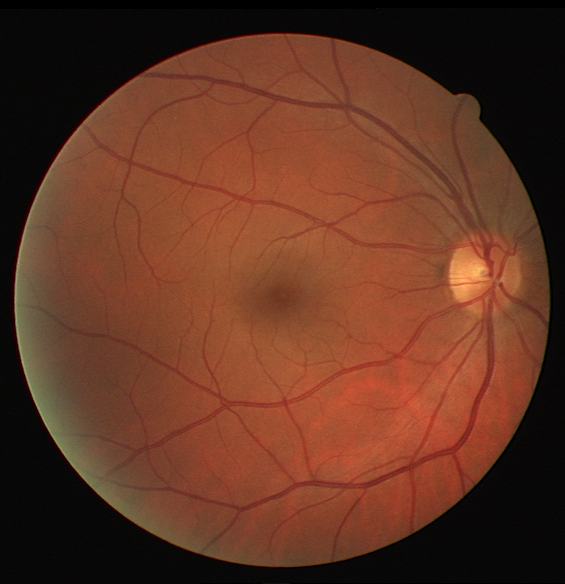
\includegraphics[width=0.18\textwidth]{figs/retina/19_DRIVE_ret} &
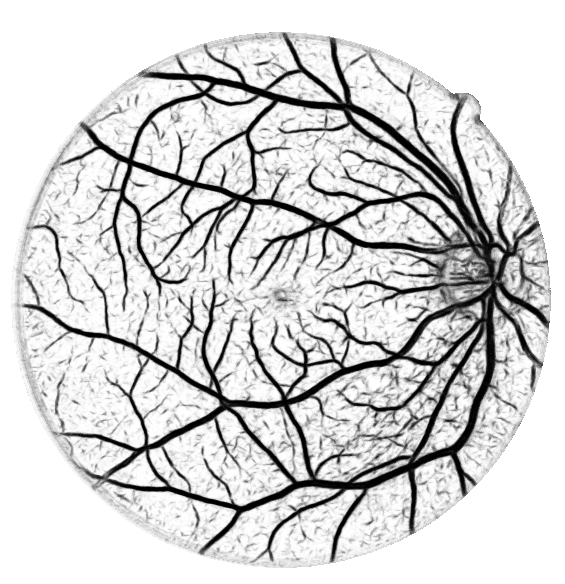
\includegraphics[width=0.18\textwidth]{figs/retina/19_DRIVE_segmentation_gabor_inv} &
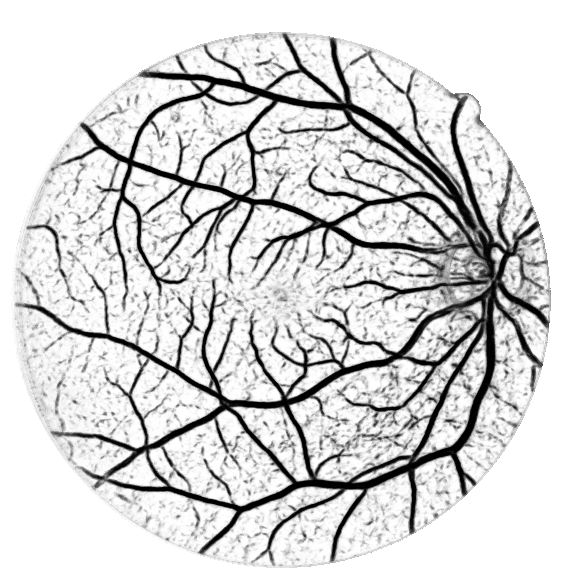
\includegraphics[width=0.18\textwidth]{figs/retina/19_DRIVE_segmentation_gh2da_inv} &
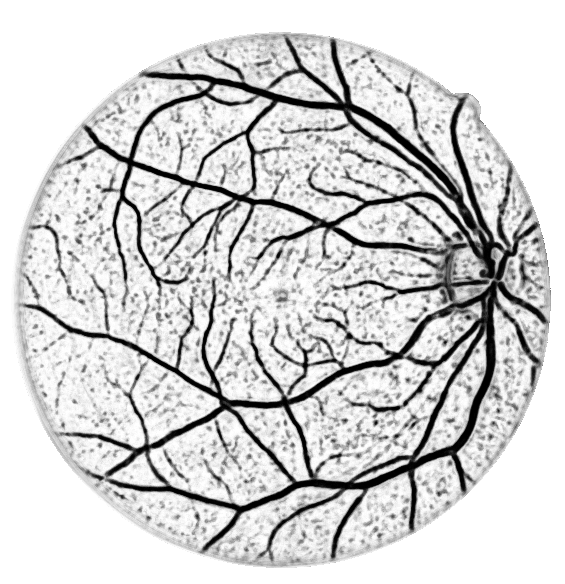
\includegraphics[width=0.18\textwidth]{figs/retina/19_DRIVE_segmentation_mono_inv} &
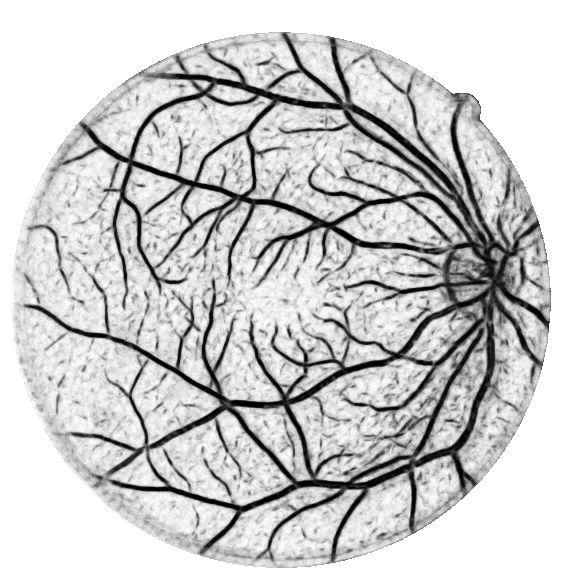
\includegraphics[width=0.18\textwidth]{figs/retina/19_DRIVE_segmentation_dt_inv} \\
(a) & (b) & (c) & (d) & (e) \\
\noalign{\smallskip}
%
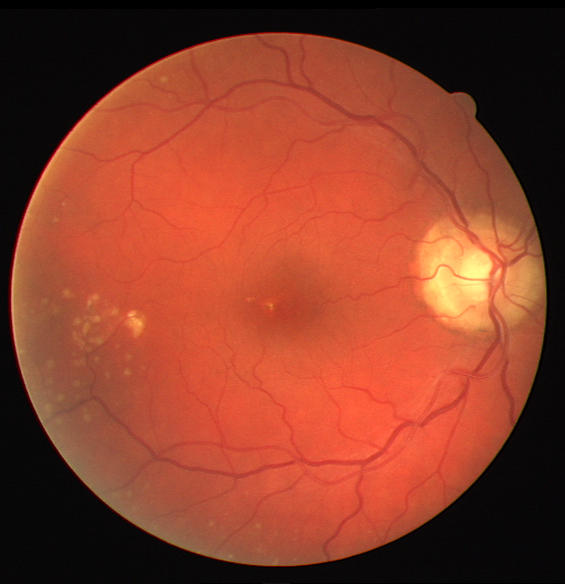
\includegraphics[width=0.18\textwidth]{figs/retina/08_DRIVE_ret} &
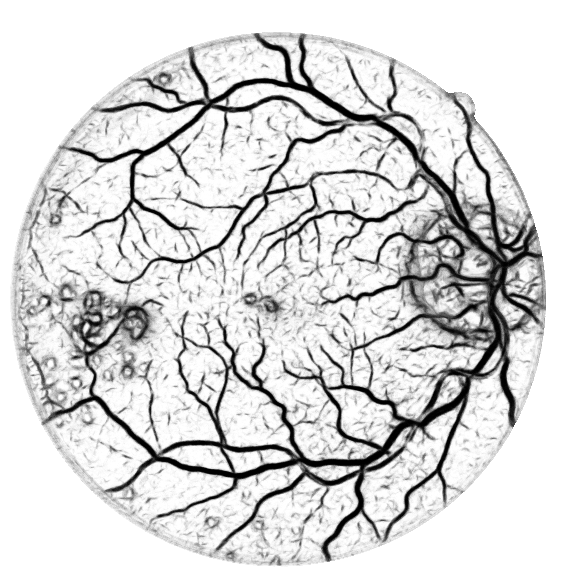
\includegraphics[width=0.18\textwidth]{figs/retina/08_DRIVE_segmentation_gabor_inv} &
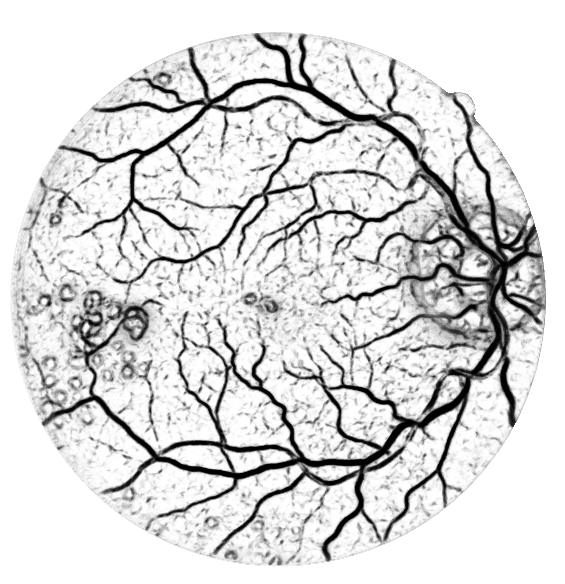
\includegraphics[width=0.18\textwidth]{figs/retina/08_DRIVE_segmentation_gh2da_inv} &
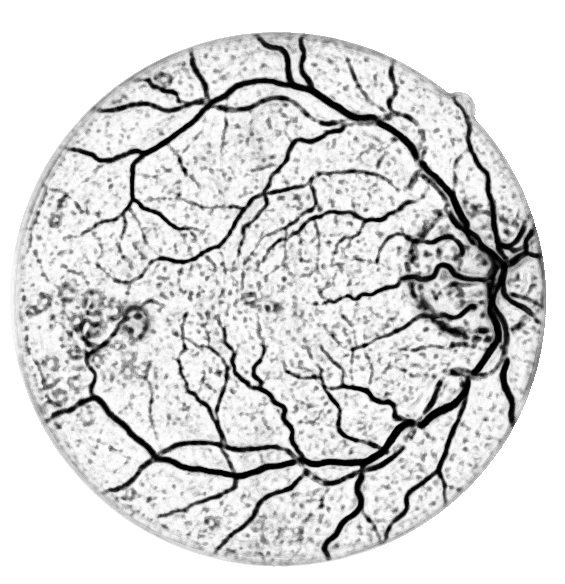
\includegraphics[width=0.18\textwidth]{figs/retina/08_DRIVE_segmentation_mono_inv} &
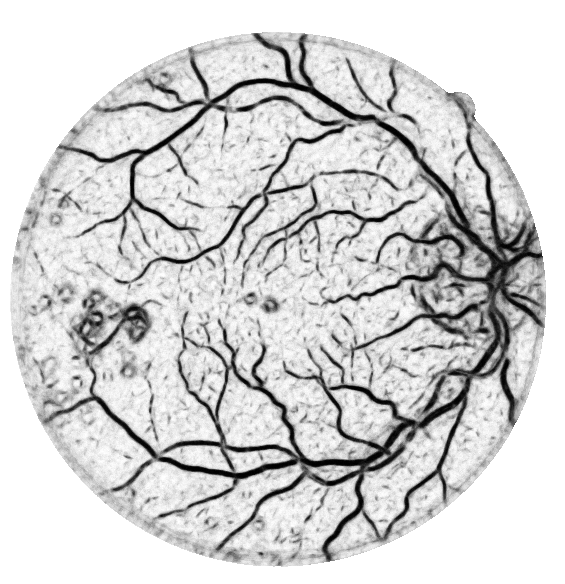
\includegraphics[width=0.18\textwidth]{figs/retina/08_DRIVE_segmentation_dt_inv} \\
(f) & (g) & (h) & (i)  & (j) \\
\noalign{\smallskip}
\end{tabular}
%
\caption{Detecting vessels in retinography: Best (a-e) and worst (f-j) results in the test set. %
(a,f) original image; %
(b,g) Gabor; %
(c,h) Gaussian; %
(d,i) Monogenic Signal; %
(e,j) \dtcwt; %
}
\label{f:drive_segmentations}
\end{figure*}
%
\begin{figure*}[t]
\centering
\begin{tabular}{@{}c c c c c@{}} % @{} removes padding around the edge of the table
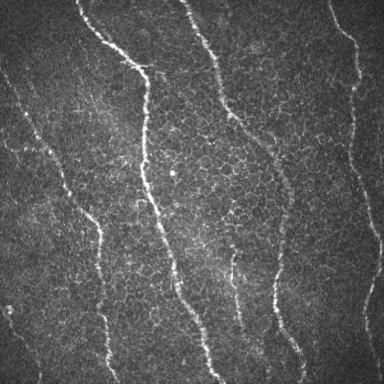
\includegraphics[width=0.18\textwidth]{figs/fibre/03_fibre_ccm} &
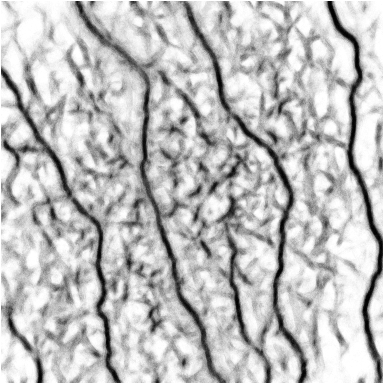
\includegraphics[width=0.18\textwidth]{figs/fibre/03_fibre_segmentation_gabor_inv} &
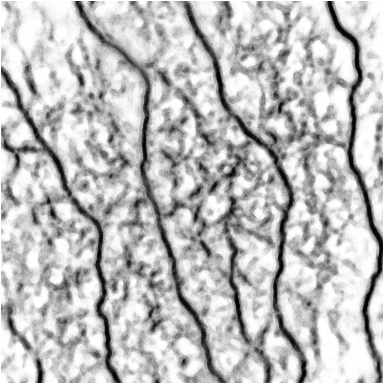
\includegraphics[width=0.18\textwidth]{figs/fibre/03_fibre_segmentation_gh2da_inv} &
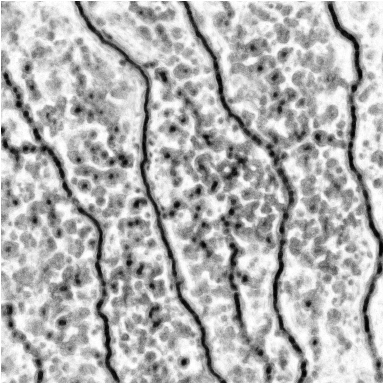
\includegraphics[width=0.18\textwidth]{figs/fibre/03_fibre_segmentation_mono_inv} &
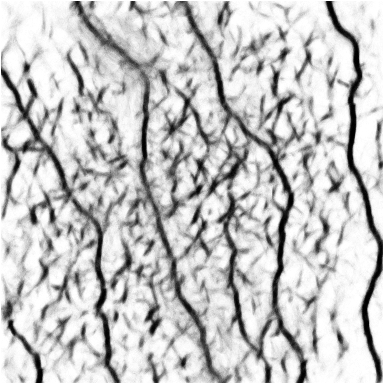
\includegraphics[width=0.18\textwidth]{figs/fibre/03_fibre_segmentation_dt_inv} \\
(a) & (b) & (c) & (d) & (e) \\
\noalign{\smallskip}
%
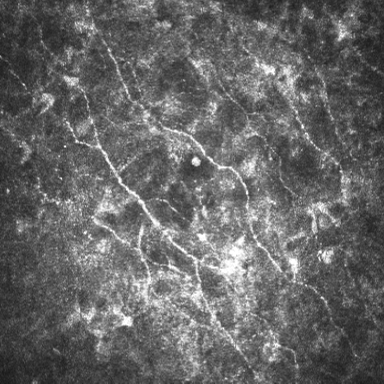
\includegraphics[width=0.18\textwidth]{figs/fibre/51_fibre_ccm} &
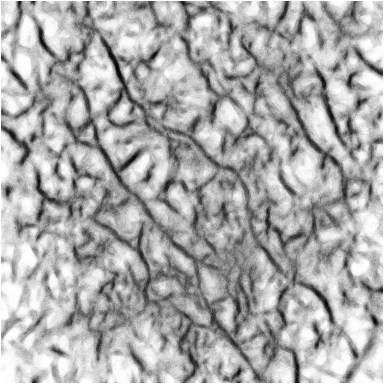
\includegraphics[width=0.18\textwidth]{figs/fibre/51_fibre_segmentation_gabor_inv} &
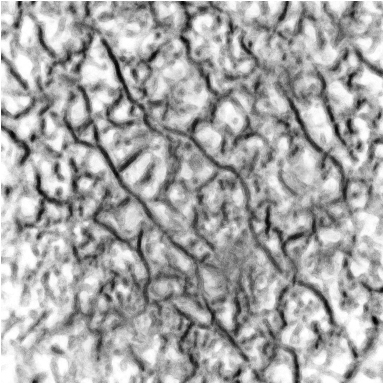
\includegraphics[width=0.18\textwidth]{figs/fibre/51_fibre_segmentation_gh2da_inv} &
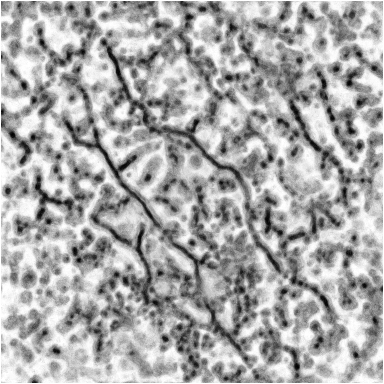
\includegraphics[width=0.18\textwidth]{figs/fibre/51_fibre_segmentation_mono_inv} &
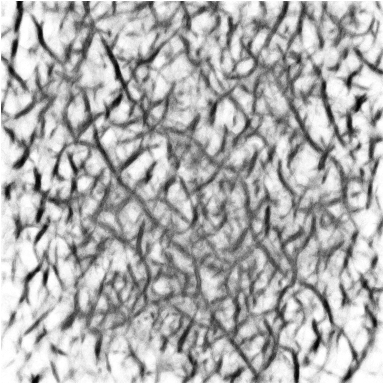
\includegraphics[width=0.18\textwidth]{figs/fibre/51_fibre_segmentation_dt_inv} \\
(f) & (g) & (h) & (i)  & (j) \\
\noalign{\smallskip}
\end{tabular}
%
\caption{Detecting fibres in CCM images: Best (a-e) and worst (f-j) results in the test set. %
(a,f) original image; %
(b,g) Gabor; %
(c,h) Gaussian; %
(d,i) Monogenic Signal; %
(e,j) \dtcwt; %
}
\label{f:fibre_segmentations}
\end{figure*}
%
%
\begin{figure}[t]
\centering
\begin{tabular}{@{}c c@{}} % @{} removes padding around the edge of the table
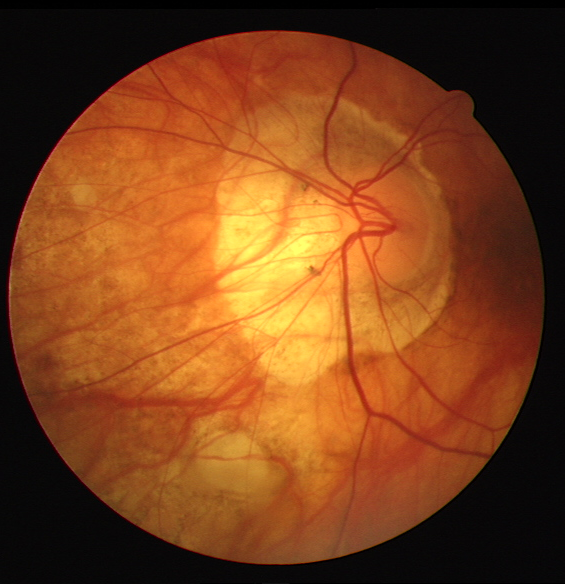
\includegraphics[width=0.48\columnwidth]{figs/retina/34_DRIVE_ret} &
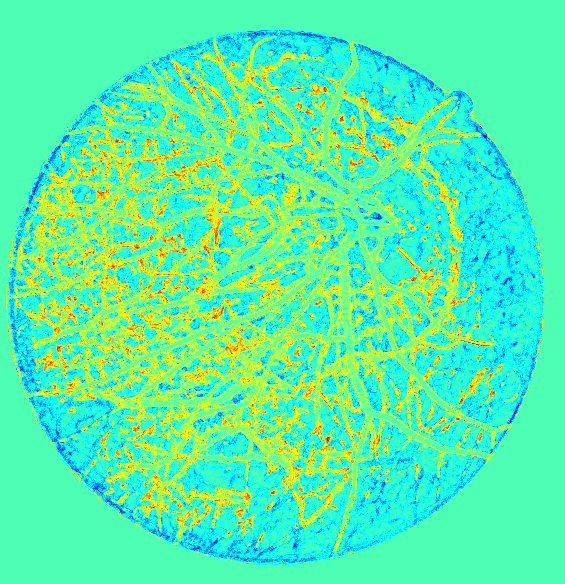
\includegraphics[width=0.48\columnwidth]{figs/retina/34_resampling_difference} \\
(a) & (b) \\
\noalign{\smallskip}
\end{tabular}
%
\caption{What effect does resampling have? %
(a) Retinogram; %
(b) Difference between prediction maps with and without resampling. Red indicates a reduced vessel probability with resampling, blue an increased vessel probability. Note the reduced prediction probability at the edge of vessels and for the false predictions caused by pathology in the image; %
}
\label{f:retinography}
\end{figure}
%
%
\begin{figure}[t]
\centering
%
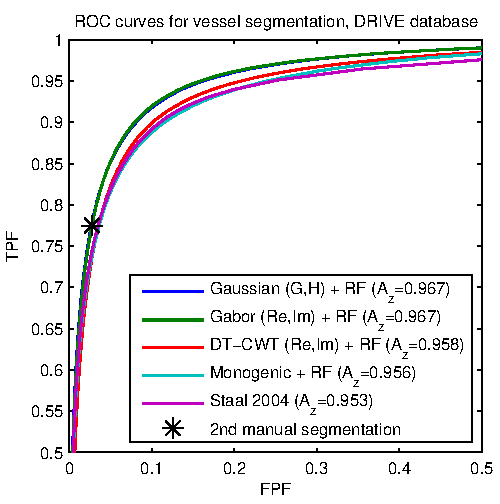
\includegraphics[width=0.9\columnwidth]{figs/retina/DRIVE_test_detection_roc_zoom}
%
\caption{Detecting vessels in retinography: DRIVE test ROCs %
}
\label{f:retinography}
\end{figure}
%
%
\begin{figure}[t]
\centering
%
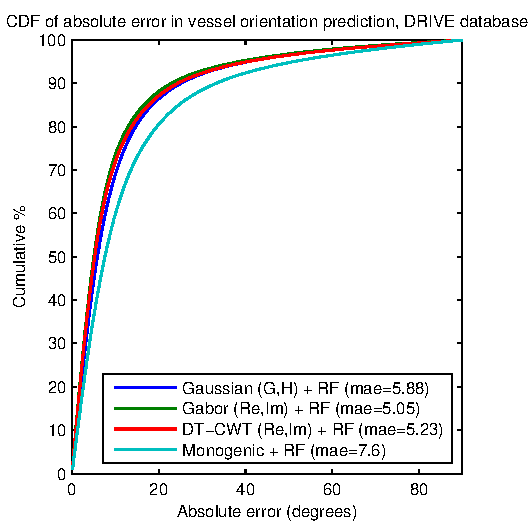
\includegraphics[width=0.9\columnwidth]{figs/retina/DRIVE_test_orientation_cdf}
%
\caption{Predicting vessel orientation in retinography: DRIVE database %
}
\label{f:retinography}
\end{figure}
%
\begin{figure}[t]
\centering
%
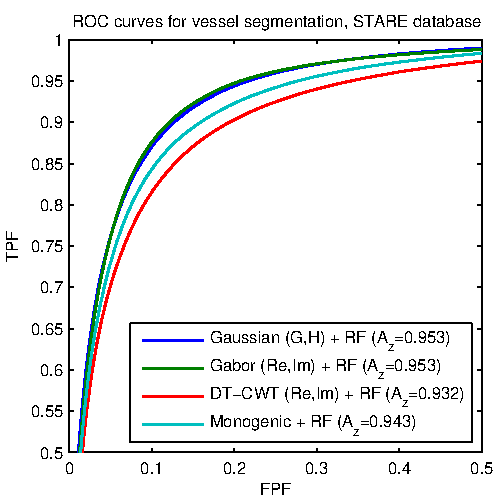
\includegraphics[width=0.9\columnwidth]{figs/retina/STARE_detection_roc_zoom}
%
\caption{Detecting vessels in retinography: STARE ROCs %
}
\label{f:retinography}
\end{figure}
%
\begin{figure}[t]
\centering
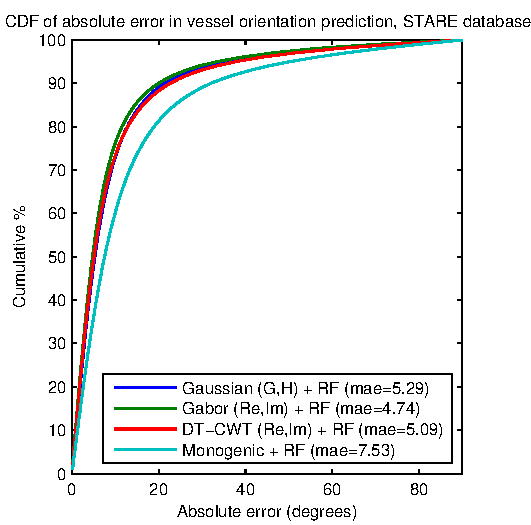
\includegraphics[width=0.9\columnwidth]{figs/retina/STARE_orientation_cdf}
%
\caption{Predicting vessel orientation in retinography: STARE database %
}
\label{f:retinography}
\end{figure}
%

\begin{itemize}
  \item DRIVE

  \begin{itemize}
    \item State of the art detection
    \item Orientation?
  \end{itemize}

  \item STARE
  \begin{itemize}
    \item Classify using DRIVE, still good performance
  \end{itemize}

  \item Fibre
  \begin{itemize}
    \item Thin and allow tolerance as per Dabbah paper
  \end{itemize}

\end{itemize}

\clearpage
\section{Discussion}

\begin{itemize}
  \item Using confidence in orientation prediction

  \begin{itemize}
    \item Possible uses
    \item Figure?
  \end{itemize}

  \item Not mentioned centreline


\end{itemize}

\label{s:discussion}

\begin{itemize}
\item Combining first and second derivatives: firsts are good at edges, seconds are good at line centres - they complement each other.

\item Discussion about linear regression coefficients: how they take a sinusoidal appearance, how we need to choose between two discrete orientations (which is not possible with a `vanilla' linear regressor)
%
\begin{figure}[t]
	\centering
		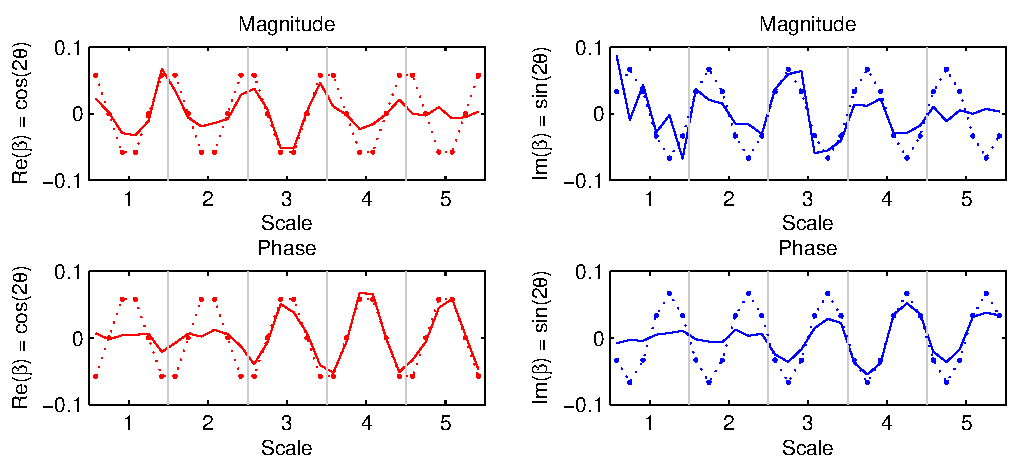
\includegraphics[width=0.9\columnwidth]{\figpath/linreg_coeffs}
	\caption{Linear regression coefficients for (left) $\cos 2\theta$ and (right) $\sin 2\theta$, using (top) response magnitude and (bottom) response phase.}
	\label{f:linreg_coeffs}
\end{figure}
%
\item Logistic regression can be used to limit the output to -1..+1. Boosted regression implicitly does the same by predicting only what it has seen before. These limits, however, are applied to sinT and cosT independently which means you can still get values outside of the unit circle.

\item Random Forest classifier/regressor has lots of details to get right, not least in making sure that the orientations wrap around correctly. Also differences in how the branches are split etc.
\end{itemize}

The results of our experimental evaluation are extremely encouraging, and represent a significant improvement over the current state of the art.

Although learning accounts for a significant part of this improvement, the choice of representation is also important and will have a different effect on performance depending on the task in hand. For example, constructing a representation based on the raw responses to Linop filters produces features that are excellent for estimating structure orientation but provide less information for determining structure shape and thus type.

Conversely, features formed from the monogenic signal are good at determining structure type - most likely because of the inclusion of the phase measure - while they perform relatively poorly at detection and orientation estimation.

For these reasons, it seems fair to conclude that the \dtcwt{} provides the best all round representation. It produced the strongest performance for all three tasks (curvilinear structure detection, orientation estimation and spicule classification). Moreover, the \dtcwt{} incurs the least overhead when working with full-size real images that require block-wise classification/regression. For example, initial tests show that the structure detection and orientation regression can be performed on a full-size (approximately $3000 \times 2400$ pixels) mammogram in approximately 1hr 30mins.

We show that, overall, our approach is significantly better than the current state-of-the-art, and that we can distinguish effectively between curvilinear structures associated with malignancy (spicules) and those associated with normal structure (vessels, ducts etc).




We have presented a discriminative learning-based approach to the detection and classification of curvilinear structures, based on a combination of \dtcwt{} representation of local structure and random forest classification. We have applied the method to the challenging problem of detecting and estimating the orientation of curvilinear structures in mammograms and distinguishing between normal and abnormal structures. The results of our experimental evaluation are extremely encouraging, and represent a significant improvement over the current state of the art.

We have also introduced learning-based variants of three existing methods, demonstrating that whilst learning accounts for a significant part of this improvement, the choice of representation is also important and will have a different effect on performance depending on the task in hand. For example, constructing a representation based on the raw responses to Linop filters produces features that are excellent for estimating structure orientation but provide less information for determining structure shape and thus type. Conversely, features formed from the monogenic signal are good at determining structure type - most likely because of the inclusion of the phase measure - whilst they perform relatively poorly at detection and orientation estimation. For these reasons, it seems fair to conclude that the \dtcwt{} provides the best all round representation. It produced the strongest performance for all three tasks (curvilinear structure detection, orientation estimation and spicule classification). Moreover, as discussed in section 5.2, of all the methods, the DT-CWT incurs the least overhead when working with full-size real images that require block-wise classification/regression. For example, initial tests show that the structure detection and orientation regression can be performed on a full-size (~3000 x 2400 pixels) mammogram in ~1hr 30mins.

Our next goal is to show that improving the individual steps of curvilinear structure and orientation estimation result in a subsequent improvement for a high level task such as detecting patterns of spiculations indicative of disease. Moreover we hope to show that classification into structure type can further aid such tasks by focusing only (or at least more) on those structures most likely to be associated with disease. 


\clearpage
\section{Conclusions}
In conclusion, we see that filters based only on odd filters perform poorly near the centre of a curvilinear structures whereas even filters such as the second derivatives are much better, though a feature set comprising the responses to both odd and even filters offers further advantages. 
There is also potential to approximate the second derivative filter responses with Haar-like features if efficiency is a key concern, though it is less clear how to combine these responses to give a unique solution. 
Of the filters we tested, we found that the \dtcwt{} gave the best results regardless of the regressor used, though was significantly more computationally expensive. Of the regressors we tested, Random Forests performed best and we have provided some insight as to why alternatives (\eg~linear regression) perform less well. 
Combining suitable filters with Random Forests produces vessel segmentation that matches the state of the art without application specific post-processing as used in rival methods (and that we would expect to improve results further). 
Moreover, we have shown that regressing orientation estimates using similar machinery is more accurate than relying on analytical estimations. 
Though demonstrated on retinograms, our methods are generally applicable to linear structures in any images where ground truth is available.
Most promisingly, we note the larger improvement in orientation estimation for particularly challenging structures such as thin, low-contrast vessels. As a further advantage of regressing with random forests, we propose that both the predicted orientation \emph{and} its associated magnitude may be useful features in further processing.
\comment{We must, however, take care when building regressors for orientation prediction in order to ensure that angles wrap around the circle correctly.}


\section*{Acknowledgements}
We thank Nick Kingsbury for the \dtcwt{} Matlab toolbox. Mammograms were provided by the Nightingale Breast Centre, South Manchester University Hospitals Trust, UK and were annotated by Dr Caroline Boggis and Dr Rumana Rahim. This work was funded by EPSRC grant EP/E031307/1.

\bibliographystyle{plain}
\bibliography{%
./bib/_aliases,%
./bib/mobio,%
./bib/mammography,%
./bib/ml,%
./bib/nailfold,%
./bib/papers_by_year,%
./bib/local}

\end{document} 